\documentclass[spanish]{template/minim}

\setmainfont{ETBembo}

%%
% For images and drawings
\usepackage{float}
\usepackage{tikz}
\usetikzlibrary{arrows,angles,positioning,shapes.misc}
\usepackage{wrapfig}
\usepackage{amssymb}
\usepackage{pgfgantt}

%%
% Better tables
\usepackage{tabularx}
\usepackage{paralist}

%%
% For euro symbol
\usepackage{eurosym}

%%
% For landscape pages
\usepackage{pdflscape}

%%
% Acronims and glossary
\renewcommand*{\glsgroupskip}{} % Captions evenly spaced
\makeglossaries{}

%%
% Code syntax highlight
\usepackage{minted}
\usemintedstyle{vs}

%%
% For empty pages
\usepackage{afterpage}

%%
% For the CC license
\usepackage[
    type={CC},
    modifier={by-nc-nd},
    version={3.0},
    ]{doclicense}

%%
% Document metadata
\usepackage[a-1b]{pdfx}

%%
% Mathematics
\usepackage{mathtools}

%%
% For multiple languages
\usepackage{babel}

% Acronyms
\newacronym{adc}{ADC}{Conversor Analógico-Digital}
\newacronym{ascii}{ASCII}{American Standard Code for Information Interchange}
\newacronym{asic}{ASIC}{Application-Specific Integrated Circuit}
\newacronym{bcd}{BCD}{Binario Codificado a Decimal}
\newacronym{bsd}{BSD}{Berkeley Software Development}
\newacronym{csv}{CSV}{Comma Separated Values}
\newacronym{cmos}{CMOS}{Complementary Metal Oxide Semiconductor}
\newacronym{dac}{DAC}{Conversor Digital-Analógico}
\newacronym{dma}{DMA}{Direct Memory Access}
\newacronym{fpga}{FPGA}{Field Programmable Gate Array}
\newacronym{gpan}{GPAN}{Generador PseudoAleatorio de Números}
\newacronym{gpl}{GPL}{GNU Product License}
\newacronym{iot}{IoT}{Internet of Things}
\newacronym{ip}{IP}{Propiedad Intelectual}
\newacronym{lut}{LUT}{Look Up Table}
\newacronym{pcb}{PCB}{Printed Circuit Board}
\newacronym{pll}{PLL}{Phase-locked loop}
\newacronym{puf}{PUF}{Physical Unclonable Function}
\newacronym{sram}{SRAM}{Static Random-Access Memory}
\newacronym{uid}{UID}{Unique IDentifier}
\newacronym{usart}{USART}{Universal Synchronous and Asynchronous Receiver-Transmitter}
\newacronym{json}{JSON}{JavaScript Object Notation}
\newacronym{ro}{RO(s)}{Ring Oscillator}


% Document metadata
\title{Control e implementación de función física inclonable en un
microprocesador}
\author{Sergio Vinagrero Gutiérrez}
\date{\today}

% Renew commands
\renewcommand{\arraystretch}{1.50}

% New commands
\newcommand{\dataelem}[1]{
    \noindent\textit{{\color{accent}{#1}}}
}

\newcommand{\blankpage}{
    \null\thispagestyle{empty}\addtocounter{page}{-1}\newpage%
}

% Bibliography file
\addbibresource{references.bib}


\begin{document}

\begin{titlepage}
\newgeometry{
    a4paper,
    left=24.8mm,
    top=27.4mm,
    headsep=2\baselineskip,     % Gap between body and header
    textwidth=107mm,
    marginparsep=8.2mm,         % Gap between body and margin notes
    marginparwidth=49.4mm,      % Width of the margin notes
    textheight=49\baselineskip, % Height of the body
    headheight=\baselineskip    % Height of the header
}

    \tikz[remember picture, overlay]
    \node[opacity=0.3,inner sep=0pt] at (current page.center){
        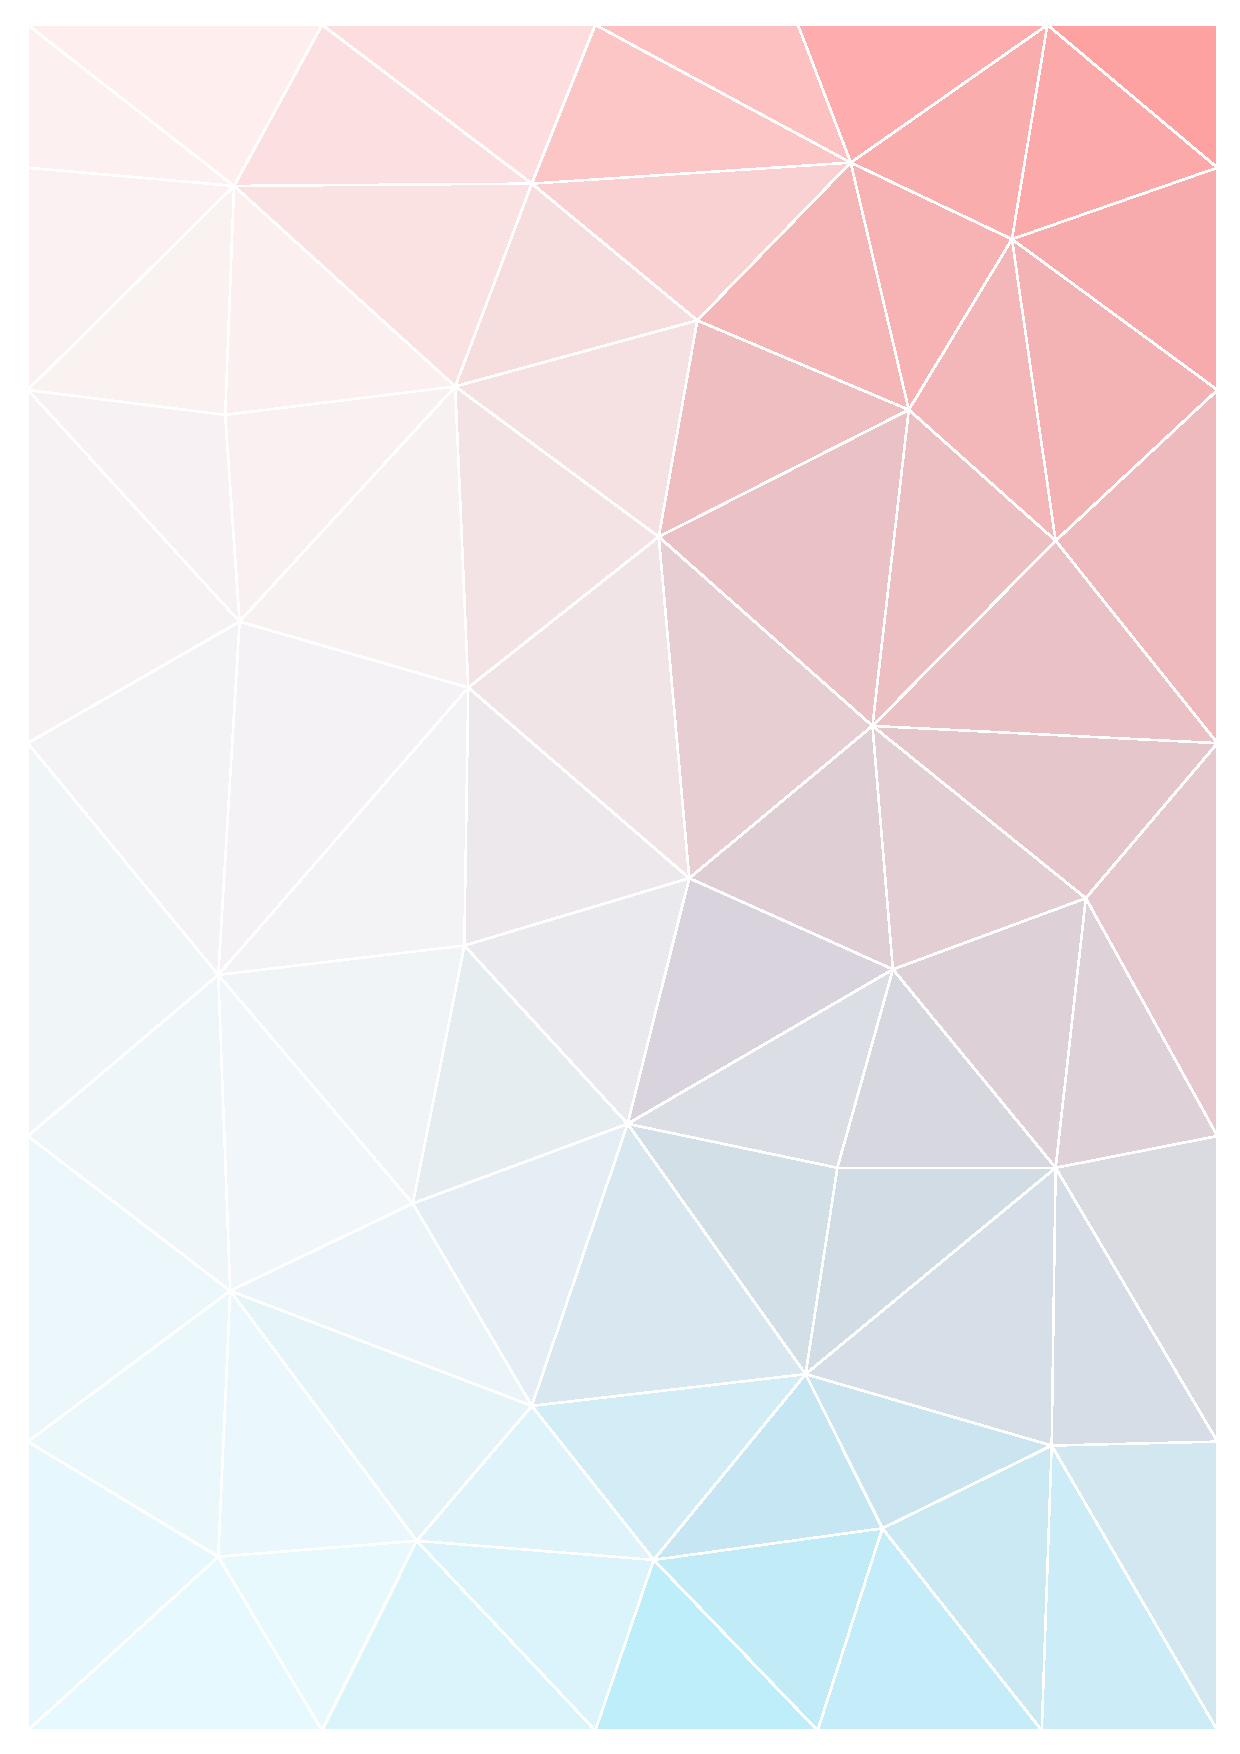
\includegraphics[width=\paperwidth,height=\paperheight]{VoronoiAlpha.pdf}
    };
    \vspace*{4cm}

    \begin{fullwidth}
        {\fontsize{22}{18}\selectfont
            \textbf{IMPLEMENTACIÓN DE UNA\\[4mm] FUNCIÓN FÍSICA INCLONABLE\\[5mm] EN UN MICROPROCESADOR}}
    \end{fullwidth}
    \vspace*{2cm}

    {\fontsize{15}{12}\selectfont Autor: Sergio Vinagrero Gutiérrez\\[3mm]Tutor: Honorio Martín González}

    \vspace*{3cm}
    \begin{fullwidth}
        {\fontsize{15}{12}\selectfont
            Trabajo Fin de Grado\\[2mm]
            Curso 2019/2020\\[2mm]
            Ingeniería Electrónica Industrial y Automática}

        \vspace*{1cm}

        {\fontsize{15}{12}\selectfont
        Universidad Carlos III De Madrid\\[2mm]
        Escuela Politécnica Superior}
    \vspace*{2cm}
    {
        \hypersetup{linkcolor=black}
        \hypersetup{hidelinks}
        \doclicenseThis{}
    }
    \end{fullwidth}

\end{titlepage}
\restoregeometry{}

\blankpage{}

\cleardoublepage{}

{
  \hypersetup{linkcolor=black}
  \hypersetup{hidelinks}
  \tableofcontents
  \listoffigures
  \listoftables
}


\cleardoublepage{}


\section{Introducción}\label{sec:introduction}

La falsificación se ha convertido en un problema creciente que ha suscitado serias preocupaciones en la industria de la electrónica en términos de impacto económico y de fiabilidad de los sistemas. Los dispositivos electrónicos no autorizados se han duplicado en los últimos 10 años. En términos económicos, la falsificación no sólo afecta a los ingresos totales de las empresas, sino que también desalienta la innovación mediante el robo de la \gls{ip}.\\

En cuanto a la fiabilidad de los sistemas electrónicos, los incidentes de piezas falsificadas encontradas en los sistemas comerciales incluyen desfibriladores, luces de aterrizaje de aeropuertos, máquinas de goteo intravenoso, sistemas de frenado para trenes de alta velocidad, e incluso la cadena de suministro para aplicaciones militares se ha visto comprometida, lo que pueden conllevar grandes problemas a la seguridad de las personas~\sidenote{Acorde a~\cite{counterfeit} la compra de componentes falsificados conlleva gastos masivos en reparación y soporte.}.\\ Por último, la seguridad de muchos sistemas, como por ejemplo los sistemas de \gls{iot}, suele basarse en las identidades de los dispositivos, por lo que la integración de circuitos falsificados puede crear vulnerabilidades y brechas de seguridad.\\

Además, el problema de la falsificación de circuitos integrados se ha visto agravado por la globalización de la industria electrónica, el coste prohibitivo de las infraestructuras necesarias para la fabricación de semiconductores y la externalización de las diferentes fases de la cadena de fabricación de circuitos integrados. Como resultado, durante la fabricación/ensamblaje se pueden enviar al mercado negro chips defectuosos, fuera de especificación o incluso sobreproducidos.\\

En este contexto, la identificación de los circuitos integrados durante toda su vida útil se ha convertido en una prioridad para la industria. Hoy en día, la identidad de los dispositivos se almacena en memorias a prueba de manipulaciones, como las memorias ROM programables y borrables eléctricamente, las Flash, o memorias que pueden ser programadas una sola vez.\\

Este enfoque tiene inconvenientes significativos relacionados con la susceptibilidad de estos tipos de memorias a los ataques físicos~\sidenote[][-2cm]{Si el identificador es almacenado en una memoria no volátil, basta con clonar la memoria y extraer el identificador de dicha copia o incluso modificarlo.}. Los identificadores actuales basados en memorias no volátiles, son vulnerables a ataques de canal lateral (side-channel attacks)~\sidenote[][2cm]{Estos ataques consisten en medir parámetros del circuito como la temperatura o radiación electromagnética para averiguar el funcionamiento del sistema.}, al uso de micro-sondas o rayos-X que permiten extraer el identificador y reprogramar un dispositivo similar de forma sencilla.\\

Una de las propuestas que más popularidad han ganado en la ultima década para solucionar los problemas que se han mencionado son las \gls{puf}, conocidas en español como funciones físicas inclonables.\\

La idea principal detrás de las funciones físicas inclonables es explotar las variaciones incontrolables que existen durante los procesos de fabricación, con el objetivo de identificar unívocamente diferentes sistemas.\\

\subsection{Objetivos}\label{sec:objectives}

El principal objetivo de este proyecto es la caracterización a gran escala de una \gls{puf} basada en memoria \gls{sram} mediante el uso de microprocesadores. Con este objetivo, el alcance del proyecto se limita a la obtención de muestras de la memoria \gls{sram} de los microprocesadores y a su posterior análisis para poder describir sus características y su funcionamiento.\\

Este objetivo principal engloba varios objetivos parciales que ayudarán a planificar el proyecto. En concreto, estos objetivos parciales consisten en:\\

\begin{itemize}
    \item {\color{accent}Creación de una estación de obtención de datos}: Se busca tener una pequeña estación que sea rápida de montar y permita la obtención de datos de las placas de la manera mas automática posible al igual que su posterior almacenamiento para los análisis. Esta estación recoge el conjunto de dispositivos necesarios y el software que se utilizará para leer y almacenar los datos.
    \item {\color{accent}Análisis de datos}: Una vez se han obtenido los datos de las placas, es necesario calcular los distintos parámetros para comprobar su funcionamiento. Estos parámetros se calcularan en base a la normativa de seguridad vigente y a los parámetros que son frecuentemente estudiados.
    \end{itemize}

    \subsection{Estructura}\label{sec:structure}

    Este documento esta estructurado de manera que en la sección~\ref{sec:introduction} se ha mostrado la motivación de este proyecto y se han expuesto los objetivos a alcanzar en este proyecto.\\

En la sección~\ref{sec:state_of_the_art} se hablará sobre las soluciones actuales que existen en el mercado para alcanzar el mismo objetivo. Se introducirá al lector acerca de las \gls{puf}, se proporcionarán los tipos de \gls{puf} más utilizadas y se profundizará en las \gls{puf} basadas en \gls{sram}. Además se muestra la normativa reguladora sobre las \gls{puf} y el impacto socio-económico que implica este proyecto.\\

En la sección~\ref{sec:planning_bill} se mostrará la planificación que se ha seguido para completar el proyecto y el coste desglosado de este.\\

En la sección~\ref{sec:setup} se expondrá el material utilizado para llevar a cabo este estudio al igual que el funcionamiento del sistema completo. El material incluye el hardware y el software necesario para extraer, almacenar y analizar la información.\\

En la sección~\ref{sec:results} se presentarán los resultados de los análisis llevados a cabo con las respuestas obtenidas de los sistemas.\\

A continuación, en la sección~\ref{sec:conclusions} se mostrarán las conclusiones sobre los resultados obtenidos seguidos de ideas que han surgido durante el desarrollo del proyecto, las cuales se detallarán en la sección~\ref{sec:lineas_futuras}.\\

Al final de este documento se incluyen una lista de acrónimos y la lista de referencias que han servido de apoyo a la escritura de este documento.\\

El texto que se encuentre en color {\color{accent}rojo} será para resaltar al lector de algo importante. El texto que se encuentre de color {\color{highlight}naranja} servirá de hipervínculo. Las citas escritas en color {\color{bleu}azul} también sirven como hipervínculos a la referencia correspondiente. En el caso de que esté viendo el documento en un medio digital, podrá utilizar los vínculos para saltar entre los distintos elementos.\\


\newpage
\section{Estado del arte}\label{sec:state_of_the_art}

Para garantizar la seguridad de los sistemas de comunicación y la creación de sistemas anti-manipulación, se utilizan herramientas de criptografía, en especial, la creación de claves criptográficas. A día de hoy existen multitud de algoritmos~\sidenote[][-1.5cm]{Estos algoritmos se conocen bajo el nombre de \textit{funciones hash criptográficas}. Los más utilizados son SHA y AES.} de generación de claves ampliamente utilizados.\\

Las soluciones más usadas hoy en día para la creación de claves criptograficas parten de la misma base: la generación de números {\color{accent}aleatorios}.\\

Sin embargo, esta no es una tarea nada fácil para máquinas deterministas que realizan las tareas en el orden en el que fueron programadas. Una de las soluciones que se ha encontrado a este problema son los generadores conocidos como \gls{gpan}. Estos generadores utilizan una {\color{accent}semilla}~\sidenote[][-1.5cm]{La semilla es el punto de partida de la secuencia. Distintas semillas producen secuencias completamente distintas unas de otras.} para generar una secuencia pseudoaleatoria de números.\\

Otra de las soluciones a este problema, en linea con las \gls{puf}, consiste en la medición de un proceso {\color{accent}físico} aleatorio. Mediante este sistema, se utiliza hardware específico para medir algún parámetro estocástico como puedan ser ruido térmico, ruido de la atmósfera o incluso de lamparas de lava~\cite{lavarand}.\\

Existen también generadores híbridos, que combinan ambos sistemas, mediante los cuales se puede utilizar una semilla junto con algún factor estocástico para generar números aleatorios.\\

Al tratarse de medios estadísticos y algoritmos, los generadores de números pseudoaleatorios son útiles para aplicaciones de uso cotidiano, ya que no es necesario un gran nivel de aleatoriedad. Sin embargo, en entornos críticos, estos sistemas presentan varios inconvenientes y es necesario utilizar la entropía de algún medio físico para generar números aleatorios que prevengan ataques de algún usuario.\\

Estos sistemas de medición de características físicas ya han encontrado su lugar en el mercado, especialmente en dispositivos integrados como FPGAs para el arranque seguro~\sidenote[][-1cm]{Estos sistemas de arranque seguro se consiguen mediante lo que se conoce como \textit{cadena de confianza}~\cite{root_of_trust}.}, como en algunos de los productos de Xilinx~\cite{zynq}.\\

Para poder identificar unívocamente cada dispositivo se puede tomar una ruta que se basa en la medición de factores aleatorios: las \gls{puf}. Como se verá más adelante, las \gls{puf} ofrecen varias ventajas a la hora de identificar dispositivos y funcionan muy bien en entornos donde se requiere un nivel de seguridad muy elevado.\\

Primero comenzaremos explicando el proceso de fabricación de circuitos electrónicos y posteriormente como se pueden explotar las características físicas de dichos circuitos para obtener los identificadores que se buscan.


\subsection{Función Física Inclonable}\label{sec:puf}

\subsubsection{Descripción}\label{sec:puf_desc}

Las \gls{puf} consisten en la generación de un identificador único para un sistema, generalmente de circuitos electrónicos, mediante la respuesta de dicho sistema a unas pruebas que miden alguna de sus características físicas. Se puede entender este funcionamiento como la generación de claves mediante una función hash criptográfica donde la semilla depende de las características intrínsecas al dispositivo.\\

Es importante marcar que estas características físicas presentan variaciones entre los distintos sistemas ya que, en el caso de circuitos electrónicos, pequeñas variaciones de temperatura o de difusión de materiales durante el proceso de fabricación hacen que no haya dos circuitos iguales. Por muy pequeñas que sean estas variaciones, como pueda ser un gradiente térmico entre dos circuitos que estén juntos en la mismo oblea, estas magnifican~\sidenote[][-.8cm]{El efecto que hace que pequeñas variaciones en la entrada produzcan grandes cambios en la salida se conoce como \textit{efecto avalancha} y es también un requerimiento de las funciones hash criptograficas.} las diferencias entre distintos sistemas, lo que hace que cada sistema sea {\color{accent}único}.\\

Como se ha comentado en el primer párrafo, no se miden estas diferencias físicas en sí, sino la manifestación de estas diferencias en el propio sistema. Esto se consigue midiendo la {\color{accent}respuesta} de cada sistema a una prueba~\sidenote[][1cm]{Estas pruebas se conocen con el nombre de {\color{accent}challenge} o {\color{accent}reto}.}. El propio sistema tiene alguna manera de medir estas variaciones, y por lo tanto el objetivo es crear un reto que sea capaz de explotar estas diferencias al máximo.\\

La idea de utilizar las características físicas de un sistema para su identificación surge en 1983 como una manera de evitar la falsificación de divisas para traspasos monetarios~\cite{bauder}. Un año más tarde se parte de ese concepto para crear un sistema genérico de identificación, no solo de dispositivos sino también de documentos y de individuos~\cite{device_identification}.

Fue a partir del nuevo milenio cuando se decidió que los sistemas midieran sus propias características, por lo que los circuitos de medición están propiamente integrados dentro del mismo circuito electrónico.\\

Gracias a que ningún sistema responde de la misma manera y que los factores físicos que crean estas diferencias son prácticamente incontrolables, su uso desde su creación ha estado fuertemente ligado a la seguridad y a la criptografía tal y como se ha visto en la sección~\ref{sec:state_of_the_art}.\\

A pesar de las ventajas que ofrecen las \gls{puf}, estas no son perfectas y presentan algunas desventajas que hay que tener en cuenta para su uso en los distintos entornos.\\

Para empezar, es necesario una manera de obtener la respuesta del sistema al reto. Esta integración suele ser costosa de diseñar y de fabricar. Este coste puede verse reducido en equipos como microcontroladores o microprocesadores que ya tienen las herramientas necesarias para medir las respuestas.\\

Por otro lado, estos sistemas tampoco se libran de posibles ataques. Los ataques con mayor probabilidad de funcionamiento son los basados en métodos predictivos, en concreto los que utilizan técnicas de aprendizaje automático como en~\cite{puf_attacks} y~\cite{puf_attacks_2}~\sidenote{También se conoce como {\color{accent}machine learning}.}. Estos ataques no solo disfrutan de la eficiencia de estos algoritmos, sino también de que son métodos que no requieren de la manipulación del dispositivo. De esta manera se puede evitar alterar el dispositivo con un manejo inadecuado lo que podría modificar la \gls{puf} y por ende bloquear el sistema de seguridad. Para mitigar los daños de estos posibles ataques, las \gls{puf} se suelen integrar dentro de sistemas de seguridad convencionales, donde el identificador generador por la \gls{puf} son un elemento más de la cadena de seguridad.\\

Además, es importante mencionar que las \gls{puf} requieren de mecanismos de código de corrección de errores para asegurar el correcto funcionamiento de estas, ya que variaciones en el entorno como cambios de temperatura o radiación electromagnética o incluso variaciones internas del hardware, pueden alterar la respuesta del sistema y por ende, obtener una respuesta que se aleja de la esperada.\\

No obstante el análisis de corrección de errores no forma parte del enfoque de este documento, por lo que en este documento solo se hablará de la obtención de la PUF en los microprocesadores.\\

Si atendemos a la manera en la que se mide la respuesta y cuántas respuestas se obtienen, podemos clasificar las \gls{puf} en varias categorías, las cuales se explicaran en la siguiente sección.\\


\subsubsection{Clasificación}

A la hora de clasificar las \gls{puf} atendiendo a la respuestas obtenidas, se suelen separar en dos grandes grupos: {\color{accent}fuertes} y {\color{accent}débiles}~\sidenote{Acorde a la normativa~\cite{ISO20897}, estos nombres se deben de sustituir por {\color{accent}extensivas} y {\color{accent}confinadas} respectivamente}. Esta separación no implica que las fuertes sean mejores que las débiles, simplemente, como reacciona el sistema ante distintas entradas. \\

Las \gls{puf} débiles se caracterizan~\cite{puf_glance} por tener un numero muy reducido de respuestas, generalmente una. Como el sistema solo tiene una respuesta, hay que asegurarse de que el acceso al reto esta restringido para que un atacante con acceso físico al dispositivo no pueda obtener la respuesta del sistema.\\

Matemáticamente, las \gls{puf} débiles se pueden expresar como una función que mapea un reto con una respuesta:

\begin{equation}
    f : \mathbb{R} \rightarrow \mathbb{R} \quad \text{donde} \quad C_i \mapsto f(C_i)
    \label{eq:weak_puf}
\end{equation}

Como las \gls{puf} débiles tienen una sola respuesta, esta se suele utilizar principalmente como clave de encriptación. La empresa que fabrica el circuito extraería la respuesta de un sistema y limitaría el acceso a la respuesta para que nadie más pueda leer la respuesta. Posteriormente se utilizaría esa clave para poder encriptar los datos que sean necesarios~\cite{puf_glance}.\\

Como se ha comentado al inicio de la sección~\ref{sec:puf}, las \gls{puf} requieren de código de corrección de errores para asegurar el correcto funcionamiento de estas. En el caso de las \gls{puf} débiles, donde la respuesta solo se extrae una vez (la empresa fabricadora del circuito) este sistema de corrección deberá estar implementado internamente para evitar una \textit{fuga}, lo cual no es algo trivial y requiere de múltiples recursos del sistema.\\\\

Por otro lado, las \gls{puf} fuertes presentan características contrarias a las débiles. Estas disponen de muchas más respuestas que las \gls{puf} débiles, ya que generalmente, suele haber más de un parámetro involucrado en la generación de la respuesta.\\

Matemáticamente, podemos expresar las PUFs fuertes mediante una función que mapea un conjunto de retos a un conjunto de respuestas:

\begin{equation}
    f : \mathbb{R}^n \rightarrow \mathbb{R}^n \quad \text{donde} \quad C_i \mapsto f(C_i)
    \label{eq:strong_puf}
\end{equation}


Una de las principales diferencias frente a las \gls{puf} débiles es que las fuertes no tienen acceso restringido de lectura de las respuestas: excepto para casos muy críticos de seguridad~\sidenote{En estos casos críticos se busca que el atacante no pueda ni tener acceso a las señales digitales que utiliza el sistema de medición, como se ve en~\cite{read_proof_hardware}.}, cualquiera con acceso físico al dispositivo puede realizar tantos retos como requiera.\\

Teniendo en cuenta que la interfaz de lectura de respuestas es fácilmente accesible, un atacante podría aprovechar esto para leer todas las respuestas. Para ello podría averiguar algunas de las respuestas e interpolarlas para averiguar el resto.\\
Sin embargo, uno de los factores críticos de las \gls{puf} fuertes es que las respuestas que generan estos sistemas son independientes y no mantienen ningún tipo de relación entre sí gracias al efecto avalancha y a las distintas características físicas que entran en juego. Si un atacante ha conseguido averiguar algunas respuestas, este no podrá utilizarlas para calcular el resto de respuestas del sistema.\\

Gracias a esta característica, las \gls{puf} fuertes son ampliamente utilizadas como sistemas de identificación. Se pueden interpretar como un sistema análogo al de las tarjetas de identificación de los bancos, donde el banco genera una serie de números aleatorios y los coloca en una tarjeta en forma de matriz. Al realizar una operación, la aplicación bancaria requiere que el usuario inserte números de dicha matriz de unas posiciones aleatorias, de esta manera, es necesario poseer la matriz entera para poder realizar una operación.\\

En este caso, este sistema se podría utilizar para identificar directamente la tarjeta: el banco generaría una lista de respuestas asociadas a cada tarjeta. Los sistemas que requieran de identificación de esta tarjeta, extraerán respuestas aleatorias del sistema y comprobarán las que se han obtenido con la lista completa que posee el banco.\\

Si atendemos a la manera en la que se puede explotar esta aleatoriedad hoy en día hay varias \gls{puf}, entre las cuales se destacan la Arbiter, la \gls{ro} y la SRAM~\gls{puf}. Comenzaremos describiendo las \gls{puf} Arbiter.\\

\myparagraph{Arbiter PUF}


En las \gls{puf} Arbiter el concepto principal es la medición del retraso de señales eléctricas por caminos similares. Como se puede ver en la imagen~\ref{fig:arbiter_puf}, estas \gls{puf} requieren de cierto número de multiplexores y un biestable al final de los caminos. Cada par de biestables se controla mediante una señal de control, por lo que hay tantas señales de control como multiplexores se deseen utilizar.\\

\begin{figure}[H]
    \centering
    \sidecaption[Arquitectura de una PUF Arbiter]{
        Arquitectura de una PUF de tipo Arbiter.~\cite{puf_arbiter}.\label{fig:arbiter_puf}
    }
    \includegraphics[width=.7\textwidth]{XORArbiter.eps}
\end{figure}

La idea detrás de este diseño es que en la realidad ninguno de esos caminos es idéntico a otro, ya que durante la fabricación de ese circuito, pequeñas variaciones aleatorias hacen que o bien los transistores que componen los componentes o las trazas que dictan los caminos de las señales eléctricas sean ligeramente diferentes, pero lo suficiente como para producir un efecto en cascada y que la respuesta cambie. Distintas configuraciones de señales de control producirán resultados distintos, al igual que las mismas configuraciones de señales de control en dispositivos distintos.\\

La palabra arbiter quiere decir \textit{arbitro} y simplemente se refiere al mecanismo utilizado para decidir que señal es la más rápida, que en el caso de la imagen esta tarea la realiza el biestable. Como a ambos caminos se les aporta la misma señal eléctrica, si la señal conectada a la entrada del biestable es más rápida, el arbitro mostrará un 1 o 0 en caso contrario.\\

Existen también variaciones de este circuito donde se tienen más de un camino de multiplexores con un biestable al final de cada camino y todos estos se conectan con una puerta lógica, normalmente una puerta OR, para producir una única salida.\\

Un aspecto positivo de este tipo de \gls{puf} es que se tienen tantas respuestas distintas como combinaciones de señales de control existan, ya que como se ha comentado, no hay dos caminos que sean exactamente idénticos. Debido a este motivo, este tipo de PUF se categoriza como una PUF fuerte.\\

\myparagraph{Ring Oscillator PUF}

Basándose en la misma idea del retraso de señales eléctricas, podemos encontrar las PUFs basadas en \gls{ro}. Se les llama osciladores ya que su salida hay una señal cuadrada que oscila entre 0 y 1. En la imagen~\ref{fig:ro_puf} podemos ver un diseño de esta \gls{puf}.\\

\begin{figure}[H]
    \centering
    \sidecaption[Arquitectura de una PUF Ring Oscillator]{
        Arquitectura de una PUF de tipo Ring Oscillator~\cite{ro_design}.\label{fig:ro_puf}
    }
    \includegraphics[width=.9\textwidth]{ROPuf.eps}
\end{figure}

Mediante esta arquitectura se pueden escoger distintas combinaciones de inversores para generar los bits que sean necesarios, de manera análoga a las señales de control de los multiplexores del caso anterior. Como cada oscilador funciona a una frecuencia ligeramente distinta, los valores de los contadores finales no serán completamente iguales y se podrá utilizar el valor de la comparación de manera similar al biestable utilizado en la \gls{puf} Arbiter.\\

Tanto la Arbiter como la \gls{ro} \gls{puf} están basadas en el mismo principio físico. El retraso de señales digitales por caminos idénticos. Sin embargo, una de las desventajas que este sistema posee es que se requieren de componentes en una configuración muy específica para su correcta utilización, aunque estos diseños son fácilmente implementables con el uso de herramientas de descripción de hardware como puedan ser Verilog o VHDL.\\

\myparagraph{SRAM PUF}

Por último, las \gls{puf} basadas en SRAM. En este último caso se intenta aprovechar las variaciones que se producen en los transistores de las memorias \gls{sram} de los microprocesadores y microcontroladores. Hoy en día las memorias \gls{sram} son ampliamente utilizadas debido a su alta velocidad de lectura y de escritura. Estas memorias se fabrican a partir de pequeñas células de memoria, las cuales son capaces de almacenar un bit de información mediante el uso de 6 transistores.\\

Para construir una memoria SRAM completa basta con reunir células de memoria hasta alcanzar el tamaño deseado. Mediante esta estructura se pueden alcanzar superficies relativamente grandes dentro del circuito lo que aumenta el efecto de las variaciones provocadas durante el proceso de fabricación. Para tener una referencia, para poder almacenar un solo kilobyte de memoria, hacen falta un total de 6144 transistores.\\

Una de las ventajas que ofrecen este tipo de \gls{puf} es que no requieren diseñar hardware adicional para aprovechar las variaciones del sistema, ya que las memorias son un sistema crítico para el correcto funcionamiento del sistema. No obstante, esto también implica que cualquier usuario con acceso al dispositivo puede leer la memoria si no se crea alguna restricción, física o lógica, de lectura y escritura.\\

Ya que este tipo de \gls{puf} es el tema central de este documento, se explicarán con mayor detalle en la sección~\ref{sec:puf_sram}.\\

Además de esta clasificación, se puede atender a la tecnología utilizada para obtener la respuesta de la \gls{puf}. Las primeras \gls{puf} se idearon en medios magnéticos y de radiofrecuencia~\cite{one_way_functions}. Posteriormente se empezaron a diseñar \gls{puf} utilizando medios ópticos y finalmente se han explorado a fondo las \gls{puf} con medios completamente electrónicos, no solo con memorias. Existen incluso diseños de \gls{puf} basados en parámetros cuánticos~\cite{quantum_puf}.\\

Antes de profundizar en las \gls{puf} basadas en memoria \gls{sram}, se mostrará como se fabrican los circuitos electrónicos para ver de donde proceden las variaciones que se han comentado.\\

\subsubsection{Fabricación de circuitos electrónicos}\label{sec:fabricacion}

Como se ha comentado brevemente en la sección anterior, el objetivo de las \gls{puf} es explotar las características físicas de naturaleza estocástica de un dispositivo para la generación de claves. En esta sección analizaremos de donde proceden estas variaciones aleatorias de los circuitos electrónicos. En la sección~\ref{sec:puf_sram} se detallarán estas variaciones para las memorias \gls{sram}.\\

El proceso de fabricación de cualquier circuito electrónico comienza con cristal de silicio. El cristal de silicio policristalino se refina para obtener un gran lingote de silicio monocristalino de gran pureza~\sidenote{Es necesario que sea un solo cristal de silicio debido a la elevada eficiencia energética y a la capacidad de dopado que presenta.}. Una vez que se tiene el lingote, este se corta con una sierra de diamante en forma de obleas con un espesor muy pequeño sobre las cuales se fabricarán los circuitos.\\

\begin{marginfigure}
    \centering
    \includegraphics[width=\textwidth]{SiliconIngot.png}
    \caption[Lingote de silicio monocristalino]{
        Lingote de cristal monocristalino expuesto en el \textit{Deutsches Museum}~\cite{silicon_crystal}. Estos lingotes pueden llegar a pesar 200 kg y tener un diámetro de 200 mm.\label{fig:silicon_ingot}}
\end{marginfigure}

El lingote de silicio se obtiene mediante una \textit{semilla} y cuarzo. Todos estos materiales se funden y se dejan enfriar hasta que forman el lingote, el cual tiene forma cilíndrica como se puede ver en la imagen~\ref{fig:silicon_ingot}. Este proceso de creación y refinado del lingote de polisilicio se controla de manera exhaustiva para cumplir con las especificaciones de calidad. Sin embargo, a lo largo de este proceso se introduce aleatoriedad en el sistema ya que por muy controlado que sea este proceso, no hay dos lugares del lingote que compartan las exactamente las mismas características físicas.\\

Este lingote se corta para formar las obleas de silicio, las cuales suelen tener un grosor más pequeño que un milímetro. Una vez se han obtenido las obleas ya se puede fabricar los transistores y componentes pasivos para crear el circuito que se requiera.\\

Para dotar al circuito de funcionalidad es necesario doparlo con metales positivos~({\color{accent}P}) y negativos~({\color{accent}N}), que generalmente suelen ser fósforo y boro respectivamente. Estos materiales dopantes permiten al polisilicio tener un exceso de {\color{accent}huecos}~\sidenote{Se conoce como huecos a la ausencia de electrones, por lo que son materiales que atraen electrones.} y de {\color{accent}electrones} respectivamente los cuales permiten el flujo de cargas eléctricas entre las distintas zonas.\\

Como se ha mencionado en este documento, los transistores hoy en día tienen un tamaño del orden de micrómetros, por lo que las técnicas convencionales de fabricación y colocación de componentes no se pueden utilizar, por lo que se utilizan técnicas de dopado especial en conjunto con técnicas de fotolitografía.\\

Con estas técnicas, se crea el circuito capa a capa. Para ello se rocía la oblea con fotoresinas y mediante el uso de luz ultravioleta~\sidenote[][1cm]{En casos muy críticos se pueden utilizar haces de electrones en vez de luz ultravioleta.} se exponen distintas máscaras a la oblea para endurecer o eliminar la fotoresina y dejar los huecos necesarios para el material dopante.\\

Actualmente existen varias procedimientos de dopado del polisilicio, pero las más utilizados son \textit{difusión} e \textit{implantación iónica}. De estos dos procesos, la difusión es el más impreciso ya que deja que el material dopante se introduzca de manera natural en el polisilicio, el cual se suele expandir a una zona mayor de la deseada. La implantación iónica es un método un poco más preciso ya que se utiliza un cañón para acelerar átomos del material dopante y bombardear la superficie de la oblea en las zonas requeridas.\\

Sin embargo, ambos métodos no son totalmente precisos e introducen aun más aleatoriedad en el sistema, ya que las zonas resultantes puede sufrir ligeras variaciones frente a los diseños originales.\\

En la siguiente sección se mostrará como afectan estas variaciones a la memorias SRAM y por tanto el tema central de este documento.


\subsubsection{PUF de SRAM}\label{sec:puf_sram}

Para el correcto funcionamiento de un microprocesador, este necesita una memoria donde pueda almacenar todo lo necesario con el código a ejecutar, como puedan ser las instrucciones, variables o datos temporales. Las instrucciones del programa se almacenan en una memoria no volátil, para que estas sigan estando en la memoria después de que se haya cortado la alimentación al dispositivo.\\

En el caso de los microprocesadores y microcontroladores, la memoria donde se almacenan las instrucciones es de tipo FLASH, debido a su alta velocidad de lectura y escritura. Esta memoria es \textit{no volátil} porque mantiene los datos después de ser desconectada de la alimentación, lo cual permite al microprocesador ejecutar el mismo código sin tener que ser reprogramado cada vez que se apaga, pero a diferencia de una memoria ROM, las memorias FLASH se pueden reprogramar tantas veces como sean necesarias.\\

Por otro lado, para almacenar las variables y datos temporales se utiliza memoria RAM, la cual es volátil, por lo que se pierden los datos que esta almacena cuando se desconecta la alimentación.\\

En función de como almacene los datos la memoria RAM, se pueden distinguir dos grandes grupos: memoria {\color{accent}estática} y memoria {\color{accent}dinámica}. La memoria estática almacena bits utilizando biestables, mientras que la memoria dinámica almacena datos mediante la carga y descarga de un transistor.\\

Esta diferencia trae consigo una serie de ventajas y de desventajas. Una de las diferencias entre ambas es que la memoria estática es varios ordenes de magnitud más rápida que la dinámica, pero a expensas de que es mucho más cara ya que requiere de un numero mayor de transistores.\\

La otra diferencia, con respecto al método de funcionamiento, es que el condensador que almacena la carga en la memoria dinámica pierde carga por corrientes parásitas por lo que es necesario \textit{refrescar} la memoria frecuentemente para poder mantener los valores. La memoria estática, al utilizar biestables no es necesario que refresque los valores, ya que los biestables no cambian de valor ni pierden la información a no ser que lo mande la señal de control.\\

En el caso de este documento estudiaremos la memoria estática o \gls{sram}. El primer paso para crear una memoria SRAM es unir un conjunto de células SRAM hasta alcanzar el tamaño de memoria deseado. Cada célula de SRAM se componen de 6 transistores para crear el biestable. Como se ha comentado en la sección~\ref{sec:fabricacion} los transistores se fabrican mediante la difusión de material dopante en el silicio, el cual adquiría distintas características en función de si era un dopante {\color{accent}P} o {\color{accent}N}.\\

Cada transistor MOSFET se compone de tres zonas diferenciadas: fuente, puerta y drenador. En función de con que dopante se realicen están zonas podemos distinguir dos tipos.\\

Por un lado, los transistores {\color{accent}N}MOS los cuales tienen el drenador y la fuente de sustrato N y la puerta de sustrato P. Esta configuración hace que al aplicar una tensión entre la puerta y la fuente, se cree un canal de tipo N en la puerta y el drenador y haya flujo de electrones desde la fuente hasta la puerta. Por lo tanto, el transistor NMOS conduce cuando está en flanco alto.\\

Por otro lado los {\color{accent}P}MOS tienen la puerta de sustrato N y el drenador y la fuente de sustrato P. Esta diferencia implica que al aplicar una tensión positiva entre la fuente y la puerta, se cree un canal P en la puerta~\sidenote{Tensión positiva entre la fuente y la puerta es lo mismo que tensión negativa entre puerta y fuente.} que permita el flujo de agujeros de la fuente al drenador. Por lo tanto, el transistor PMOS conduce cuanto está en flanco bajo.\\

Como se puede ver, ambos tipos de transistores presentan funcionamientos {\color{accent}complementarios}. Se pueden aprovechar estas diferencias mediante lo que se conoce como \gls{cmos}. Mediante esta tecnología ambos transistores son utilizados de manera complementaria para realizar cualquier puerta lógica.\\

Debido a esto se dobla el numero de transistores necesarios para hacer la mayoría de puertas lógicas, pero los dispositivos fabricados utilizando esta tecnología tienen muy bajo consumo, ya que los transistores NMOS y PMOS solo consumen cuando están conmutando y no tienen perdidas pasivas~\sidenote{Debido a corrientes parásitas y al pequeño tamaño de los transistores existen pequeñas perdidas pasivas.} Este bajo consumo es ideal para microprocesadores, dispositivos portátiles o cualquier otro dispositivo electrónico que sea alimentado con una batería.\\

Con esto en mente, mostraremos un diseño de una célula de SRAM fabricada utilizando tecnología \gls{cmos}. En la imagen~\ref{fig:cmos_sram} podemos ver los 6 transistores necesarios para crear la célula. La señal de control del biestable es $WL$ y la lectura y escritura se controla mediante las líneas $BL$ y $\overline{BL}$.\\

\begin{figure}[H]
    \centering
    \sidecaption[Célula de SRAM con tecnología CMOS]{
        Célula de SRAM utilizando 6 transistores. Los transistores $M_2$ y $M_4$ son de tipo PMOS y el resto de transistores son de tipo NMOS. BL representa la \textit{Bit Line} y WL representa la \textit{Word Line}.\label{fig:cmos_sram}
    }
    \includegraphics[width=.7\textwidth]{CMOSSRAM.eps}
\end{figure}

Se ha comentado en la sección~\ref{sec:fabricacion} que los procesos de fabricación de transistores para esos tamaños son muy sensibles a factores externos como puedan ser la temperatura o la humedad del ambiente. Además, los procesos de dopado de los metales para la creación de las distintas zonas de los transistores no son perfectos, por lo que existe una pequeña difusión de dopante no controlada en el transistor.\\

Estos factores son críticos a la hora de explotar las características físicas de la memoria SRAM ya que estas variaciones, aunque sean ínfimas, son suficientes para cambiar las proporciones de las distintas zonas y por consiguiente, variar las tensiones umbrales a la que los transistores conmutarían. En el caso de la célula de SRAM que se ha enseñado, esto implica que la célula tienda hacia un valor positivo o negativo. A gran escala esto implica que la memoria SRAM no se ponga completamente a cero durante el proceso de reset, sino que muestre un sesgo de valores y esto en esencia es como se obtiene la \gls{puf} de la memoria SRAM.\\

Es de crítica importancia exponer que para poder obtener correctamente la respuesta de la memoria SRAM, hay que desconectar la alimentación y conectarla de nuevo; no es suficiente con provocar un reset, ya sea por hardware o por software. Esto es así ya que el reset pone los valores de la memoria a cero, pero es durante la conexión de la alimentación que las variaciones de los tamaños de los transistores hacen que se produzca el sesgo que altera los valores de la memoria. Si solo se hiciese un reset \textit{lógico} no se estarían leyendo los valores que caracterizarían a ese dispositivo.\\

Como las variaciones durante el proceso de fabricación no son sistemáticas y no hay dos circuitos que compartan exactamente las mismas características físicas por muy cerca que estén, no habrá dos placas que compartan el mismo sesgo y por tanto mostrarán respuestas distintas.\\

Es importante marcar que las \gls{puf} generadas utilizando la memoria SRAM son de naturaleza débil, ya que el sistema solo presenta una respuesta ante la lectura de la memoria.\\

Un aspecto positivo de las \gls{puf} basadas en \gls{sram} es que la memoria RAM de los microprocesadores ya viene incorporada en el dispositivo, porque es un elemento crítico para el funcionamiento correcto del microprocesador. Además los mecanismos de lectura y escritura de la memoria también son están disponibles fácilmente.\\

\subsubsection{Aplicaciones}

Como se ha comentado anteriormente, las \gls{puf} son utilizadas en entornos que requieren una seguridad muy elevada y en aplicaciones de criptografía.\\

Si tomamos por ejemplo la creación de claves criptograficas, las \gls{puf} pueden generar sistemas más seguros que con la manera ordinaria de creación de claves. Como la clave se puede generar a partir de la respuesta del sistema a través de un reto, esta no tiene porqué estar en memoria previamente para ser utilizada, simplemente se puede medir la respuesta cada vez que sea necesario. Cuanto más tiempo esté la clave en memoria, más tiempo tiene un atacante de averiguar cual podría ser esta clave~\sidenote{No solo un atacante podría leer la clave, sino que podría forzar la memoria con determinados valores para que el programa crea que esta leyendo una clave legitima.}, por lo que reducir este tiempo, incluso si es posible eliminarlo completamente, es una gran ventaja frente a ataques de lectura de memoria.\\

El hecho de que la clave no permanezca en memoria es en sí es otra ventaja, ya que hay algunas \gls{puf} que son muy sensibles a la manipulación, por lo que un atacante con acceso físico al dispositivo podría romper la cadena de generación de claves al manejar dicho dispositivo de una manera inadecuada.\\

Otro uso para el que las \gls{puf} están sobrepasando a otros sistemas, es la identificación de dispositivos, especialmente en entornos como \gls{iot}. Los dispositivos que funcionan en este entorno suelen funcionar con baterías, por lo que hay que reducir el consumo sustancialmente. Los sistemas de comunicaciones complejos requieren de sistemas de encriptación complejos los cuales pueden suponer una carga computacional alta y por tanto un consumo elevado.\\

Las \gls{puf} suponen una alternativa a los medios convencionales ya que en la mayoría de los casos los sistemas de medición de las respuestas suelen estar integrados dentro de los dispositivos y las claves generadas no abandonan el sistema digital, por lo que se puede aumentar el nivel de seguridad mientras que se mantiene un bajo consumo.\\

\subsection{Impacto socio-económico}

Se ha comentado al comienzo del documento que las \gls{puf} están ganando terreno en las alternativas a los sistemas de seguridad convencionales. Mediante este estudio se obtendrán datos que aportaran información sobre su comportamiento en sistemas de grandes dimensiones, los cuales son idóneos para usos en entornos como \gls{iot}.\\

Los datos que se obtengan de los estudios realizados en este proyecto proporcionarán información sobre las memorias sram de los microprocesadores, los cuales permitirán reducir los costes de la creación y el mantenimiento de los nuevos sistemas de seguridad y de identificación. No solo se conseguirán reducciones en coste, sino que los parámetros obtenidos en este estudio permitirán explotar a fondo las propiedades de las \gls{puf} para la creación de sistemas de seguridad más robustos que los actuales o para la creación de protocolos de comunicación mas transparentes y fiables.\\

\subsection{Marco regulador}\label{sec:norm}

\subsubsection{Normativa}

A día de hoy la única normativa existente relacionada con las \gls{puf} es la ISO/IEC DIS 20897~\cite{ISO20897}. Esta normativa se divide en dos partes: ISO/IEC DIS 20897-1 e ISO/IEC DIS 20897-2. La primera se refiere a los requerimientos de seguridad de las \gls{puf} para su uso en diferentes entornos y la segunda sienta las bases para los métodos de pruebas y de evaluación de resultados.\\

Estos estándares se centran en el uso de las \gls{puf} como sistemas de seguridad sin necesidad de uso de memoria para almacenar claves y debido a eso establecen ciertos parámetros que la \gls{puf} debe de cumplir para poder ser utilizada.\\

No obstante, hay que tener en cuenta que ambos estándares están aun en desarrollo. Debido a esto, este documento se centrará específicamente en los parámetros analíticos de la \gls{puf}.\\


\subsubsection{Propiedad intelectual}

En la sección~\ref{sec:bill} se ha mencionado que el coste del desarrollo de la programación de las placas es de cero euros ya que las tecnologías utilizadas son gratuitas.\\

Las herramientas utilizadas para el análisis de datos, en concreto R~\cite{r} y Python~\cite{python}, poseen licencias de código abierto. R esta licenciado bajo las licencias \gls{bsd}~\cite{bsd} y \gls{gpl}~\cite{gpl} mientras que Python esta licenciado bajo su propia licencia, la cual es compatible con \gls{gpl}. Además, las librerías utilizadas proporcionadas por STM para programar los microcontroladores están licenciadas también bajo la licencia \gls{bsd}.\\

Empezando por la licencia mas restrictiva, la licencia \gls{gpl}, permite el libre uso, distribución y modificación del código, pero a cambio el usuario esta obligado a publicar los cambios que haya realizado al código original. Por otro lado, la licencia \gls{bsd} es mas laxa y no tiene estas restricciones. Con esta licencia el usuario no está obligado a publicar los cambios que haga al código, aunque es una buena práctica hacerlo, e incluso puede convertir el código original en un producto privado. Sin embargo, bajo esta licencia el autor original no es responsable de los problemas que pueda causar el código utilizado.\\

Hay que resaltar también que ambas licencias comparten un comportamiento \textit{vírico}: las modificaciones que hagamos al código deberán ser publicadas bajo la misma licencia, por lo que si se modificasen las librerías de STM y quisiésemos publicar los cambios, tendríamos que hacerlo bajo licencia \gls{bsd}.\\

En resumen, este proyecto no se ve afectado por la propiedad intelectual de las herramientas utilizadas para realizarlo, sino todo lo contrario, ya que se dispone de plena libertad para utilizar las herramientas.\\

Además de las herramientas utilizadas, el trabajo realizado durante este proyecto se ha ido almacenando en la plataforma github~\cite{github} continuamente para mantener siempre una copia del estado del proyecto. Todo este trabajo está disponible en el repositorio \url{https://github.com/servinagrero/Bachelor_Thesis}. Como se ha mencionado en la sección anterior, no hay que pagar mantenimiento de los servidores ya que mantener las aplicaciones y el código utilizado en esta plataforma no conlleva ningún coste para el usuario.\\

Debido a los motivos que se han mostrado en el párrafo anterior, el trabajo publicado en el repositorio se encuentra licenciado bajo \gls{gpl}, para que cualquiera pueda hacer uso de estos datos y tenga la obligación de publicar los cambios que realice, como una manera de incentivar la innovación y la mejora de esta investigación.\\

\section{Planificación y presupuesto}\label{sec:planning_bill}

\subsection{Planificación}\label{sec:planning}

Para la planificación de este proyecto se han tenido en cuenta las restricciones internas y externas, siendo las externas las impuestas por la universidad. Las más limitantes para el desarrollo del proyecto han sido:

\begin{itemize}
\item Máximo de 360 horas de trabajo acorde al plan Bolonia y a los 12 créditos ECTS que corresponden al trabajo de fin de grado.~\sidenote{Cada crédito se corresponde con 30 horas de trabajo.}
\item La fecha de entrega del proyecto se establece para el día 3 de julio de 2020.
\item Las placas de desarrollo utilizadas para la toma de datos son utilizadas por los estudiantes del grado en ingeniería en tecnologías de telecomunicación en el segundo cuatrimestre. Esto implica que no se tendrá acceso a las placas a partir del 27 de enero de 2020, por lo que cualquier parte del proyecto que necesite las placas deberá concluirse antes de esa fecha.
\end{itemize}

Con estas restricciones en mente, se comenzó a trabajar en este proyecto al comienzo del primer cuatrimestre, con fecha de 4 de septiembre de 2019. Como la fecha limite de entrega de la memoria del proyecto es el 3 de julio de 2020, eso nos da un total de 43 semanas para la ejecución del proyecto incluyendo la memoria. Estas 43 semanas se han repartido entre las siguientes partes del proyecto.\\

Primero se estudiaron las necesidades del proyecto y se contrastaron con el hardware disponible. Se tuvieron que estudiar completamente las características de las placas para ver como se podían obtener los datos de la memoria SRAM y de los sensores de temperatura y de tensión. Se buscó también una manera de identificar las placas para poder identificarlas durante los análisis~\sidenote{Se buscaba simplemente poder asignar a cada placa un código para saber de que placa procedía cada muestra. Como se verá más adelante, STM aporta estas herramientas en los kits.}. Después se buscó una manera de poder almacenar todos los datos que se fueran a obtener. Debido a la gran cantidad de datos que se iban a obtener se optó por buscar una base de datos fácil que utilizar para poder organizar todas las muestras.\\

Posteriormente fue necesario el desarrollo del código para el funcionamiento de las placas. En esta etapa se ha creado el código de funcionamiento de las placas al igual que los scripts necesarios para la lectura de dichos datos y su almacenamiento en la base de datos. Se incluye aquí también la configuración y el diseño de la base de datos. Durante esta etapa, las pruebas de funcionamiento han tomado una gran parte del tiempo: no solo se han corregido los errores de software y de la estación hardware sino que también se ha ido creando varias iteraciones del código de recolección de muestras para obtener resultados de manera más sencilla y más rápidamente. Esta etapa ha concluido una vez que el estado del software de toma de datos y la estación hardware están en un punto que permiten la correcta y rápida obtención de gran cantidad de datos de varias placas.\\

Una vez se ha desarrollado todo el software necesario y se ha comprobado su funcionamiento se ha procedido a la toma de datos. Como se ha comentado al comienzo de esta sección, todos los datos se deben de tomar antes del 27 de enero de 2020~\sidenote{En esta fecha comienza el segundo cuatrimestre académico.}. Para ello se concretaron fechas en las que se tomarían los datos de todas las placas, ya que como las placas son propiedad de la universidad, solo se puede hacer uso de ellas cuando los técnicos del laboratorio nos lo permitan. Cada sesión de recolección de datos duró aproximadamente dos horas y media. A pesar de que se realizaron solo 8 sesiones para la toma de datos, las cuales suponen un total de 20 horas, estas se han espaciado en un periodo de 3 meses comenzando en noviembre y acabando en enero.\\

Una vez se han tomado todas las muestras se ha procedido al análisis de los resultados. Primeramente, es necesario el desarrollo de programas y scripts para la conversión y análisis de los parámetros necesarios. Estos programas se iban creando secuencialmente una vez se había concluido el análisis de un parámetro. Durante esta etapa, el cálculo de los parámetros ha sido el factor limitante ya que debido a la gran cantidad de datos de los que se dispone, los cálculos se realizaron a lo largo de dos semanas. Por otro lado, el desarrollo de los programas de análisis se realizo a lo largo de tres semanas.\\

Todo esto queda resumido en el siguiente diagrama de Gantt~\sidenote[][-2.5cm]{Como se ha comentado, muchas tareas del proyecto se han realizado en muy pocas sesiones pero espaciadas en un gran periodo de tiempo.}.\\

\begin{fullwidth}
    \definecolor{barblue}{RGB}{153,204,254}
    \definecolor{groupblue}{RGB}{51,102,254}
    \definecolor{linkred}{RGB}{165,0,33}
    \renewcommand\sfdefault{phv}
    \renewcommand\mddefault{mc}
    \renewcommand\bfdefault{bc}
    \centering

    \begin{figure}[H]
    \centering
    \setganttlinklabel{s-s}{}
    \begin{ganttchart}[
        vgrid,
        fractional xshift/.style={%
            /tikz/xshift=#1*\pgfkeysvalueof{/pgfgantt/x unit},
        },
        canvas/.append style={fill=none, draw=black!10, line width=.5pt},
        include title in canvas=false,
        group peaks tip position=0,
        group label node/.append style={left=.5cm},
        group label font=\bfseries\small,
        group/.append style={draw=none, fill=red!90!black!50},
        group incomplete/.append style={fill=groupblue},
        group left shift=0,
        group right shift=0,
        group height=.5,
        title/.style={draw=none, fill=none},
        title label font=\bfseries\footnotesize,
        title label node/.append style={above=1pt},
        bar label font=\mdseries\small\color{black!100},
        bar label node/.append style={left=.5cm},
        bar/.append style={draw=none, fill=barblue},
        bar incomplete/.append style={fill=barblue},
        bar progress label font=\mdseries\footnotesize\color{black!70},
        hgrid style/.style={draw=black!5, line width=.75pt},
        vgrid={*1{draw=black!5, line width=.75pt}},
        x unit=9mm,
        time slot format={isodate},
        time slot unit=month
        ]{2019-09-04}{2020-07-03}
        \gantttitlecalendar{year, month=shortname} \\
        \ganttgroup{Programación de placas}{2019-09-04}{2019-10-30} \\
        \ganttbar{Software microprocesadores}{2019-09-04}{2019-09-15} \\
        \ganttbar{Programa adquisición datos}{2019-09-15}{2019-09-21} \\
        \ganttbar{Pruebas funcionamiento}{2019-10-01}{2019-10-30} \\\\
        \ganttgroup{Toma de datos}{2019-11-01}{2020-01-30} \\
        \ganttbar{Ajustes del sistema}{2019-11-01}{2019-11-30} \\
        \ganttbar{Extracción de datos}{2019-11-30}{2020-01-30} \\\\
        \ganttgroup{Análisis}{2020-02-01}{2020-05-00} \\
        \ganttbar{Software para análisis}{2020-02-01}{2020-02-28} \\
        \ganttbar{Calculo de parámetros}{2020-03-01}{2020-03-28} \\
        \ganttbar{Análisis de datos}{2020-04-01}{2020-04-30} \\\\
        \ganttgroup{Memoria}{2020-05-00}{2020-07-30} \\
        \ganttbar{Redacción}{2020-05-00}{2020-07-30} \\
\end{ganttchart}

    \caption[Planificación del proyecto]{
        Diagrama de Gantt con la planificación del proyecto. Elaboración propia.\label{fig:gantt_plan}
    }
    \end{figure}
    \end{fullwidth}

\subsection{Presupuesto}\label{sec:bill}

El coste total del proyecto se ha calculado teniendo en cuenta los tres aspectos fundamentales de este: hardware, software y personal.\\

Para el coste del personal, se han dividido las tareas necesarias en los distintos cargos que realizarían dicha tarea, en base a las tareas mostradas en el diagrama de Gantt. Para obtener una estimación del coste del cada cargo se ha obtenido el salario medio anual en España mediante~\cite{glassdoor} y se ha convertido el sueldo por año a sueldo por hora utilizando~\cite{calcxml}. Con estos datos y las horas extraídas del diagrama~\ref{fig:gantt_plan} se ha obtenido el coste total del personal.\\

Se ha mencionado que el proyecto supone un máximo de 360 horas de trabajo. De esas 360 horas en esta tabla solo quedan recogidas 100 horas. Estas 100 horas son las que se han utilizado para programar todo el software y analizar todos los datos. No se han incluido aquí las horas de diseño, ni de pruebas de funcionamiento ni de búsqueda de información.\\


\begin{table}[H]
    \centering
    \sidecaption[Coste del personal del proyecto]{
        Coste del personal del proyecto.\label{tab:bill_people}
    }
    \begin{tabularx}{\textwidth}{Xrrr}
      \toprule
      \multicolumn{4}{c}{Coste del personal del proyecto} \\
      \midrule
      Cargo & Horas & Salario/h (\euro{}) & Total (\euro{}) \\
      \midrule
      Desarrollador software & 20 & 15,31 & 306,20 \\
      Analista & 80 & 20,67 & 1653,60 \\
      \midrule
      Total & & & 1959,80\\
      \bottomrule
    \end{tabularx}
\end{table}


En cuanto al coste del software tenemos que tener en cuenta los aspectos de costes de desarrollo y de mantenimiento. Tanto las herramientas proporcionadas por STM como las utilizadas para el análisis de datos son libres, no hay que pagar ninguna licencia. Además, la base de datos se ha mantenido en el ordenador en el que se tomaron las muestras, por lo que no ha sido necesario pagar el mantenimiento de un servidor web. Todo esto implica que no hay gastos de software.\\


\begin{table}[H]
    \centering
    \sidecaption[Coste del software del proyecto]{
        Coste del software del proyecto.\label{tab:bill_software}
    }
    \begin{tabularx}{\textwidth}{Xrrr}
      \toprule
      \multicolumn{4}{c}{Coste del software del proyecto} \\
      \midrule
      Concepto & Unidades & Coste/Ud (\euro{}) & Total (\euro{}) \\
      \midrule
      Total & & & 0,00\\
      \bottomrule
    \end{tabularx}
\end{table}


Para el cálculo del coste del hardware se ha utilizado la configuración final establecida para la toma de datos. Para el coste del ordenador, se ha tenido en cuenta las especificaciones mínimas necesarias para la programación y el análisis de datos. Actualmente, cualquier ordenador de gama baja dispone de especificaciones suficientes como para llevar a cabo estas tareas, por lo que se han omitido sus especificaciones técnicas.\\

\begin{table}[H]
    \centering
    \sidecaption[Coste del hardware del proyecto]{
        Coste del hardware del proyecto. Solo se han tenido en cuenta el coste de 5 placas de desarrollo para la realización de pruebas, cuando en realidad se han obtenido muestras de 206 placas.\label{tab:bill_hardware}
    }
    \begin{tabularx}{\textwidth}{Xrrr}
      \toprule
      \multicolumn{4}{c}{Coste del hardware del proyecto} \\
      \midrule
      Concepto & Ud & Coste/Ud (\euro{}) & Total (\euro{}) \\
      \midrule
      Hub USB programable & 1 & 34,99 & 34,99 \\
      Hub USB & 1 & 7,99 & 7,99 \\
      Placas de desarrollo* & 5 & 12,50 & 62,50 \\
      Ordenador & 1 & 300,00 & 300,00 \\
      Transductor FT232 & 3 & 5,99 & 17,97 \\
      Cable USB & 1 & 2,99 & 2,99 \\
      \midrule
      Total & & & 426,44 \\
      \bottomrule
    \end{tabularx}
\end{table}


Con toda esta información, el coste total del proyecto asciende a DOS MIL TRESCIENTOS OCHENTA Y SEIS EUROS CON 24 CÉNTIMOS (2386,24 \euro{})~\sidenote{El coste total incluye impuestos}, el cual queda resumido en la siguiente tabla.\\

\begin{table}[H]
    \centering
    \sidecaption[Coste total del proyecto]{
        Coste total del proyecto.\label{tab:bill_total}
    }
    \begin{tabularx}{\textwidth}{Xr}
      \toprule
      \multicolumn{2}{c}{Coste total del proyecto} \\
      \midrule
      Concepto & Coste (\euro{}) \\
      \midrule
      Coste de software & 0,00 \\
      Coste de hardware & 426,44 \\
      Coste de personal & 1959,80 \\
      \midrule
      Total & 2386,24 \\
      \bottomrule
    \end{tabularx}
\end{table}


\section{Equipo utilizado}\label{sec:setup}

En esta sección se detallará el material utilizado para la extracción de las respuestas de los sistemas.\\

El sistema propuesto para el estudio de la función física inclonable se ha dividido en hardware y software. Dentro del software se ha hecho la distinción entre programación del hardware, extracción de las respuestas de los sistemas y almacenamiento de los paquetes de datos.\\

\subsection{Hardware}\label{sec:desc_boards}

\begin{marginfigure}
    \centering
    \includegraphics[width=.7\textwidth]{board.png}
    \caption[Placa de desarrollo 32L152C-DISCOVERY]{
        Placa de desarrollo 32L152C-DISCOVERY. Las especificaciones completas del kit se encuentran en su hoja de características~\cite{discovery}.\label{fig:board}}
\end{marginfigure}

Para el estudio se han utilizado los kits 32L152C-DISCOVERY, de la empresa STM. Se disponen de un gran número de estas placas, ya que son utilizadas por el estudiantado.\\

Esta placa de desarrollo se fabrica en dos modelos, dependiendo del microprocesador elegido. Para este estudio se ha dispuesto de ambos modelos, el STM32L152RBT6 y el STM32L152RCT6. Ambas placas son idénticas a nivel físico. La única diferencia es a nivel lógico, en el microprocesador que utilizan.\\

Para facilitar el seguimiento de este estudio, se utilizarán alias para referirse a estos dos modelos de placas de desarrollo. Se nombrarán los modelos STM32L152R{\color{accent}B}T6 como modelo {\color{accent}32} y las STM32L152R{\color{accent}C}T6 como {\color{accent}64}. El motivo de estos alias se expondrá más adelante, pero está directamente relacionado con la memoria \gls{sram}.\\

En cuanto al número de placas, se ha dispuesto aproximadamente del mismo número para ambos modelos: {\color{accent}91} placas para el modelo {\color{accent}32} y {\color{accent}115} para el modelo {\color{accent}64}, lo que hacen un total de {\color{accent}206} placas.\\

\begin{marginfigure}
    \centering
    \includegraphics[width=1.4\textwidth]{YKUSH.png}
    \caption[Hub programable YKUSH]{Hub programable YKUSH de Yepkit. Las especificaciones completas del hub se encuentran en su hoja de características~\cite{yepkit}.\label{fig:YKUSH}}
\end{marginfigure}


El último dispositivo que se ha utilizado para obtener las respuestas de los sistemas es un hub programable. El modelo utilizado es YKUSH de Yepkit. El único objetivo de esta placa es permitir el encendido y apagado simultáneo de múltiples placas en paralelo, que en el caso del sistema final han sido tres.\\

\subsubsection{Especificaciones técnicas}\label{sec:spec_boards}

En esta sección solo se mostrarán las especificaciones técnicas de las placas de desarrollo utilizadas, dado que son el elemento clave en este estudio.\\

Son de principal importancia las características de las distintas memorias, en especial la memoria \gls{sram}. El resto de especificaciones como la tensión de alimentación o la frecuencia del reloj serán tomadas como variables de control.\\

Los microprocesadores utilizados mostrados en la sección~\ref{sec:desc_boards} se pueden encontrar en otras placas de desarrollo, montadas sobre una \gls{pcb} distinta, por lo que podrían mostrar un comportamiento diferente del mostrado en este documento. Es por esto, que el estudio propuesto será aplicable a las placas utilizadas.\\

No obstante, distintas placas no deberían mostrar un comportamiento diferente ya que la memoria de estos microprocesadores esta integrada en el mismo encapsulado, por lo que deberían de mostrarse impasibles ante estímulos externos, como periféricos de entrada-salida.\\

Para empezar, ambos modelos presentan una arquitectura de 32 bits. El resto de información se muestra en la siguiente tabla:

\begin{table}[H]
    \sidecaption[Especificaciones técnicas]{
        Especificaciones técnicas de ambos modelos de placas utilizadas. La frecuencia base del reloj es de 32 KHz, pero se puede aumentar a 32 MHz. Las especificaciones completas de ambos modelos se encuentran en sus respectivas hojas de características~\cite{discovery}.\label{fig:spec_boards}
    }%

    \begin{tabularx}{\textwidth}{Xr@{\hspace{2cm}}r}
      \toprule
      Especificación & Placa 32 & Placa 64 \\
      \midrule
      Flash & 128 KB & 256 KB\\
      E2PROM & 4 KB & 8 KB  \\
      SRAM & 16 KB & 32 KB \\
      $V_{DD}$ & 1.65 a 3.6 V & 1.65 a 3.6 V \\
      $T_{MIN}$ & -40 $^\circ$C & -40 $^\circ$C\\
      $T_{MAX}$ & 105 $^\circ$C & 105 $^\circ$C \\
      $f_{CLK}$ & 32 MHz & 32 MHz\\
      DAC & 12 bits & 12 bits \\
      ADC & 12 bits & 12 bits \\
      \bottomrule
    \end{tabularx}

\end{table}

Como se puede ver en la tabla~\ref{fig:spec_boards}, el modelo 64 dispone del doble de memoria que el modelo 32. De esta manera, se estudiará el efecto que tiene el tamaño de la memoria a la hora de generar las \gls{puf}, aunque no se disponga de información sobre la estructura física de la memoria.\\

Estos kits disponen de más periféricos adicionales como un sensor táctil, una pantalla LCD y dos botones. Dichos periféricos no se tendrán en cuenta y permanecerán desactivados durante las tomas de datos al no tener implicación directa con el estudio propuesto.

\subsection{Paquetes de datos}\label{sec:desc_packet}

Para extraer la respuesta de la memoria \gls{sram} de cada placa, se han programado las placas para enviar paquetes mediante comunicación \gls{usart} con los campos que se mostraran a continuación.\\

\dataelem{ID}\\
Identificador de 12 bytes de cada muestra. Esta representado con 24 caracteres alfanuméricos. Sirve únicamente para identificar cada muestra en la base de datos. Este identificador es asignado por la base de datos al guardar el paquete y es único, por lo que 2 muestras no pueden tener el mismo identificador, incluso si el contenido que tienen es idéntico.\\

\dataelem{UID del microprocesador}\\
Identificador de 96 bits guardado en la memoria del microprocesador por la empresa que ha fabricado los microprocesadores para identificar las placas.\\

Este identificador se encuentra en la zona de memoria {\color{accent}0x1FF80050} para las placas de modelo 32 y en la {\color{accent}0x1FF800D0} para las de 64. En la hoja de características de las placas esta zona de memoria aparece marcada como `bytes de opciones'.

Los 96 bits de \gls{uid} codifican la siguiente información, acorde a~\cite{stm32_registers}:

\begin{itemize}
    \item[] \textit{\color{accent}{Oblea}}\\
        Byte para la oblea de silicio a la que pertenecía el microprocesador.
    \item[] \textit{\color{accent}{Lote}}\\
        7 bytes en código \gls{ascii} para el número de lote del microprocesador.
    \item[] \textit{\color{accent}{X}}\\
        2 bytes en \gls{bcd} para la coordenada X del microprocesador en la oblea.
    \item[] \textit{\color{accent}{Y}}\\
        2 bytes en BCD para la coordenada Y del microprocesador en la oblea.
\end{itemize}

Cabe destacar la disposición de los 96 bits en las direcciones proporcionadas, ya que no se encuentran en una secuencia lineal. Empezando en la posición indicada, se encuentra el byte de la oblea, los 7 bytes del lote y a tras un offset de 20 bytes, los últimos 4 bytes de las coordenadas.\\

\dataelem{Tipo}\\
Este valor será de 32 para las placas de modelo 32 y 64 para el modelo 64. Este identificador coincide con el alias del modelo de la placa.\\ Permite discernir las muestras de las placas de un modelo en la base de datos y en los scripts sin tener que recurrir a la zona de memoria.\\

\dataelem{Región de memoria}\\
Número de 28 bytes en notación hexadecimal que indica la región de memoria donde empieza la muestra. La memoria \gls{sram} de ambos modelos de placa comienza en la dirección {\color{Red}0x20000000}.\\

Se ha escogido utilizar muestras de 512 bytes ya que es un número lo suficientemente pequeño como para poder analizar la memoria SRAM con precisión pero lo suficientemente grande como para facilitar los análisis. Para almacenar la memoria de cada placa son necesarias 32 muestras para las placas de modelo 32 y 64 muestras para las del modelo 64. Este es el motivo de los alias que se han dado a los dos modelos, ya que es altamente distintivo.\\

\dataelem{Temperatura}\\
Temperatura interna, en grados Celsius, del microprocesador en el tiempo en el que se ha tomado la medida. Para poder obtener la temperatura en grados Celsius, primero hay que medir la salida del canal de temperatura del \gls{adc}. Se obtiene el valor en tensión del conversor, por lo que es necesario utilizar los valores de calibración que se mostrarán a continuación para calcular la temperatura real.\\

\dataelem{Vdd}\\
Tensión de alimentación de la placa. Se obtiene también gracias al conversor analógico digital y al valor de calibración que se muestra más adelante. Se obtiene la tensión a la que funciona el conversor analógico digital, que es proporcional a la tensión de alimentación del dispositivo.

\dataelem{Marca de tiempo}\\
Año, mes, día, hora, minuto y segundo de cuándo se ha obtenido la muestra. Debido a la velocidad de comunicación de las placas con el ordenador y el tamaño de cada muestra, 2 muestras consecutivas se realizan con segundos de diferencia, por lo que cada muestra tiene una marca de tiempo única. Esto permitirá analizar el comportamiento de la memoria SRAM en el tiempo.\\

\dataelem{Tensión de calibración a 30 grados}\\
Tensión de calibración del conversor analógico digital que debe mostrar a la salida cuando se encuentra a 30 grados. Este dato se encuentra guardado en la región {\color{accent}0x1FF8007A} para las placas del modelo 32 y {\color{accent}0x1FF800FA} para las del modelo 64.\\

\dataelem{Tensión de calibración a 110 grados}\\
Dato de calibración análogo al anterior, excepto que ahora el valor es para cuando la placa alcance 110 grados Celsius. Este dato se encuentra en la región {\color{accent}0x1FF8007E} para las placas del modelo 32 y {\color{accent}0x1FF800FE} para las del modelo 64.\\

\dataelem{Tensión de calibración del sensor de tensión}\\
Dato de calibración del canal de tensión del conversor analógico digital. Permite medir la tensión de funcionamiento de la placa midiendo la tensión de funcionamiento del conversor analógico digital, ya que ambas tensiones están directamente relacionadas. Este dato se encuentra en la región {\color{accent}0x1FF80078} para las placas del modelo 32 y {\color{accent}0x1FF800F8} para las del modelo 64.\\

\dataelem{Datos}\\
Lista de 512 bytes de respuesta del sistema. Se almacena en la base de datos como una lista de 512 números enteros que van desde 0 hasta 255. Posteriormente, se procederá a convertir esta lista de 512 números a otra lista de 4096 bits, representados como 0 o 1, para el análisis bit a bit, lo cual aportara mucha mas información en los análisis futuros.\\

Para el estudio propuesto se han almacenado un mínimo de 25 muestras de cada zona de memoria por cada placa, lo que resulta en un total de aproximadamente 260.000 muestras, las cuales ocupan un tamaño de aproximadamente 5 GB en la base de datos. Se explicara con mas detalle en la sección~\ref{sec:database} el almacenamiento de las respuestas en la base de datos.\\

A la hora de trasmitir la respuesta del sistema, se ha decidido transmitir los bytes, a pesar de que los análisis posteriores se realizan a nivel de bit, para agilizar la transmisión de información. Una vez se han obtenido todas las muestras se pueden convertir fácilmente los bytes a bits directamente en la base de datos o mediante el uso de Python.\\

Con esta configuración, se puede descargar la memoria entera de una placa en un rango de aproximadamente 2 a 4 segundos, dependiendo del modelo de placa, por lo que las 25 muestras toman menos de 2 minutos.\\


\subsubsection{Temperatura de referencia}
Para obtener la temperatura real de funcionamiento del sistema, debemos disponer de 3 valores: los 2 valores de calibración y la medida del conversor. Utilizando la siguiente fórmula, calculamos la temperatura de funcionamiento.\\

\begin{figure}[H]
    \centering
        \sidecaption[Cálculo de la temperatura de funcionamiento]{
            Cálculo de la temperatura de funcionamiento. Los valores $T_{CAL 30}$ y $T_{CAL 110}$ se han fijado a 680 mV y a 858 mV respectivamente extrapolando los datos de todas las placas.\label{eq:temperature}
        }%

        \begin{align*}
          T_{REAL} = m \cdot t + 30.0~\si{\celsius}\\[.8em]
          t = T_{ADC} - T_{CAL 30}~\si{\milli\volt}\\[.8em]
          m = \frac{110 - 30}{T_{CAL 110} - T_{CAL 30}}~\si{\celsius\per\milli\volt}
        \end{align*}

\end{figure}

De esta manera obtenemos una pendiente en la recta de calibración de $0.5$ \si{\celsius}/mV, el cual no es valor muy elevado teniendo en cuenta que el conversor analógico digital tiene 12 bits. Sin embargo, la recta se ha realizado para dos valores extremos muy distantes, por lo que en la zona de funcionamiento, cercana a los 30 \si{\celsius} obtenemos muy poca resolución.\\

Es necesario señalar la presencia de un problema con los valores de calibración de las placas. A pesar de que estos valores están en zonas reservadas de solo lectura, algunas placas, especialmente las del modelo 32 no mantenían estos valores, por lo que los valores de calibración son igual a 0. Más adelante se mostrara como se ha solventado este problema.\\

La primera explicación es que debido al frecuente uso de estas placas por los estudiantes, se han borrado estos valores por un uso indebido de estas o por las programaciones frecuentes que sufren.\\

Como se toman varias muestras sucesivamente, es posible que exista un ligero aumento de la temperatura de la placa debido al uso continuado de la USART y del ADC. También puede haber fluctuaciones de temperatura debido a los tiempos de apagado y encendido de cada placa. Es por estos motivos por los que se decidió almacenar la temperatura de la placa en cada muestra. No obstante, en nuestro caso no se han obtenido variaciones significativas.\\

En cuanto a la temperatura ambiente, se ha realizado el experimento en la misma sala y franja horaria, para evitar fluctuaciones en los datos debidas a estas características. Teniendo esto en cuenta, los valores de temperatura que se han obtenido están en el rango de 35 \si{\celsius} a 40 \si{\celsius}.\\

\subsubsection{Tensión de referencia}\label{sec:vdd_reference}

Se muestra a continuación el cálculo de la tensión de funcionamiento real del sistema. Para ello, al igual que con la temperatura, son necesarios el valor de calibración del sensor de tensión y el valor medido por el conversor analógico digital.

\begin{figure}[H]
    \sidecaption[Cálculo de la tensión de funcionamiento][-1cm]{
        Cálculo de la tensión de funcionamiento. El cociente es el porcentaje de alimentación que la placa recibe con respecto a la tensión de referencia, los 3.3 V. El valor de $V_{INT CAL}$ se ha fijado a 1666.\label{eq:vdd}
    }%

    \begin{equation*}
        V_{DD} = 3.3 \cdot \frac{V_{INT CAL}}{V_{INT DATA}}
    \end{equation*}

\end{figure}

La salida del sensor de tensión se conecta directamente al pin $ADC\_17$ del conversor analógico digital, para ambos modelos de placas. Por lo que solo es necesario dividir la tensión de calibración entre la tensión medida.\\

Se ha mencionado en la tabla~\ref{fig:spec_boards} que la tensión de funcionamiento de ambos modelos permite 3.6 V. No obstante, los conversores están conectados directamente a un diodo, el cual los mantiene a 3.3 V para evitar errores debido a fluctuaciones en la alimentación del sistema.\\

Con un análisis superficial de las muestras, vemos que estas se realizaron con una tensión de alimentación muy cercana a la tensión fijada por el fabricante, entre 3.25 V y 3.3 V. Se profundizara en la sección~\ref{sec:metadata_results} el estudio de estas dos variables.\\

No obstante y ateniendo a los resultados obtenidos, se puede presentar la hipótesis de que los valores que se han obtenido están en el rango de funcionamiento fijado por el fabricante, por lo que los resultados de los análisis deberían de ser los esperados para el funcionamiento ordinario de los sistemas.\\

En contraste, hay variables de control que no se han tenido en cuenta para el análisis y han podido tener una gran influencia en los resultados, como pueda ser la radiación electromagnética producida por la red eléctrica o interferencias de dispositivos cercanos a los utilizados mientras se obtenían las muestras.\\

Como se ha visto en las ecuaciones~\ref{eq:temperature} y~\ref{eq:vdd}, las curvas de calibración se realizan con valores muy extremos, por lo que en el rango de funcionamiento usual de las placan no se dispone de mucha resolución. Se puede utilizar esto para solventar el problema de la falta de valores de calibración de algunas placas.\\

En los datos obtenidos, se observa que los valores de calibración son prácticamente idénticos, por lo que podemos extrapolar la temperatura y la tensión real de los sistemas que no disponen de estos datos con los valores de calibración medios y fijar sus valores medios en las fórmulas para el cálculo de la temperatura y la tensión.


\subsection{Software}\label{sec:programming}

En esta sección se detallará la programación y configuración de los microprocesadores para obtener los datos necesarios para el estudio propuesto.\\

Se dividirá este sección en la configuración de los periféricos de ambos modelos de placas y en el desarrollo del programa principal para la creación y extracción de los paquetes de datos.

\subsubsection{Configuración de periféricos}\label{sec:config_boards}

Los periféricos de los que se han dispuesto para extraer los datos de las placas son el conversor analógico digital, el \gls{dma} y el puerto \gls{usart} para la comunicación con el ordenador.\\

La empresa STM32 dispone del software STM32CubeMx, el cual incorpora una interfaz gráfica para configurar los parámetros de los periféricos de manera muy precisa.\\

Se puntualizarán a continuación los parámetros de configuración de cada periférico.\\

\dataelem{Puerto USART}

Los kits utilizados disponen de un controlador de comunicación \gls{usart} y de un puerto USB.\\

Estas placas disponen de hasta 3 puertos USART. Se ha utilizado el USART2 ya que este puerto tiene mapeados pines, los cuales se pueden conectar fácilmente a otro dispositivo mediante jumpers.\\

\begin{table}[h]
    \centering

    \sidecaption[Configuración del puerto USART][-10mm]{
        Parámetros de configuración del puerto USART. Los valores de esta tabla se han obtenido directamente de STM32CubeMx.
        \label{fig:usart_config}
    }%

    \begin{tabular}{p{4cm}r}
        \toprule
        Parámetro & Valor \\
        \midrule
        Modo & Asíncrono \\
        Baudios & 350.000\\
        Ancho de palabra & 8 Bits\\
        Paridad & Ninguna\\
        Bit de parada & 1\\
        \bottomrule
    \end{tabular}

\end{table}

No obstante, estas placas no poseen un transductor de \gls{usart} a USB, por lo que es necesario utilizar uno externo para poder comunicar las placas con el ordenador. El transductor utilizado es el {\color{Red}FT232} debido a su alta disponibilidad y facilidad de uso.\\

El transductor dispone de 4 pines: VDD, GND, TXD y RXD. Los pines de VDD y GND del transductor se conectan a los respectivos pines de VDD y GND de la placa. Los pines TXD y RXD se conectan a los pines PA2 y PA3 que se encuentran en los extremos laterales de las placas.\\

Los pines PA2 y PA3 son los pines que están configurados por defecto para el USART2. En caso de que estos pines se encuentren en uso, podemos modificar el mapeado de pines del USART2 mediante la herramienta STM32CubeMx.\\

El conector USB se conecta al único puerto USB del que dispone la placa, situado en el extremo superior de esta.\\

\dataelem{DMA}

El \gls{dma}, permite acceder a la memoria principal del microprocesador de manera independiente. El único propósito de este sistema es la recolección automática de datos del \gls{adc}.\\

En las siguientes tablas se muestran los parámetros de configuración del \gls{dma}. Los valores de esta tabla se han obtenido directamente de STM32CubeMx.\\

\begin{table}[h]
    \centering
        \sidecaption[Primera configuración del DMA]{
        Parámetros de configuración del DMA. Se puede acceder a estos parámetros desde la pestaña del DMA o desde la pestaña de configuración del \gls{adc}, en el submenu de configuración del DMA.~\label{fig:dma_config}
    }%

    \begin{tabularx}{\linewidth}{Xrr}
        \toprule
        Petición & Canal & Dirección \\
        \midrule
        ADC & DMA Canal 1 & Periférico a memoria \\
        \bottomrule
        Modo & Ancho de dato P & Ancho de dato M \\
        \midrule
        Circular & Palabra & Palabra \\
        \bottomrule
    \end{tabularx}

\end{table}

Es importante mencionar que el \gls{dma} solo ha sido utilizado para las placas del modelos 32. Las placas del modelo 64 se añadieron al proyecto cuando gran parte del software ya estaba desarrollado.\\

Asimismo, las placas del modelo 64 presentaron muchos problemas al configurar el DMA por lo que se tuvo que optar por otra solución, explicada en el siguiente periférico, para no alterar el progreso realizado.\\

La solución por la que se ha optado no supone un gran distanciamiento frente al sistema original, por lo que no debería de suponer una gran diferencia entre ambos sistemas.\\

\dataelem{Conversor Analógico Digital}

Como se ha mencionado anteriormente, el \gls{adc} tiene el único propósito de obtener datos de los sensores. Por eso solo se han utilizado los canales del sensor de temperatura y de Vrefint, el sensor de tensión.\\


\begin{table}[H]
    \centering

    \sidecaption[Configuración del ADC]{
        Parámetros de configuración del \gls{adc} y de sus respectivos canales. El parámetro de Trigger Externo aparece en el selector de canales. Los valores de esta tabla se han obtenido directamente de STM32CubeMx.~\label{fig:adc_config}
    }%

    \begin{tabularx}{\linewidth}{Xr}
        \toprule
        Parámetro & Valor \\
        \midrule
        Preescalado & 1\\
        Resolución & 12 bits\\
        Alineamiento & A la derecha\\
        Escaneo & Activado\\
        Modo continuo & Activado\\
        Modo discontinuo & Desactivado\\
        DMA Continuous request & Activado\\
        Fin Conversión & Una conversión\\
        Espera Low Power & Desactivado\\
        Apagado Low Power & Desactivado\\
        \midrule
        Num. Conversiones & 2\\
        Trigger Externo & Software\\
        Nivel de Trigger & Ninguno\\
        Canal & Vrefint\\
        Canal & Temperatura\\
        \bottomrule
    \end{tabularx}

\end{table}

Los parámetros de configuración mostrados en la tabla~\ref{fig:adc_config} son comunes a ambos modelos de placas.\\

Los parámetros de la tabla~\ref{fig:adc_config} solo se han utilizado para el modelo 32, ya que es este modelo el que hace uso del DMA.\\

Para las placas del modelo 64, se ha creado una copia de la estructura de configuración del periférico y se ha cambiado el canal de lectura de datos.\\

\dataelem{RCC}

Esta sección corresponde a la configuración del reloj de la placa, ya que ambos sistemas disponen de un \gls{pll}, el cual es un sistema diseñado para modificar la frecuencia de reloj base.\\

Esta configuración se encuentra en la herramienta, en la pestaña de `Configuración del reloj' y en la pestaña de configuración `RCC'.\\

La frecuencia base del reloj es de 32~KHz. Sin embargo, se ha utilizado 32~MHz, la frecuencia máxima de funcionamiento del sistema. Se ha escogido este valor para agilizar todo el proceso de recolección de datos.\\


\subsubsection{Programa principal}\label{sec:main_program}

El objetivo del programa principal es leer los sensores y las zonas de memoria necesarios, crear los paquetes de datos y enviarlos secuencialmente por el puerto serie para que sean recibidos y almacenados por el ordenador.\\

El programa se ha desarrollado en C utilizando las librerías disponibles de STM para el desarrollo de aplicaciones en sus microprocesadores.\\

Es importante aclarar que debido a ciertas diferencias entre ambas placas, los periféricos no están configurados de la misma manera, ni los punteros apuntan a las mismas direcciones de memoria. No obstante ambos códigos consiguen el mismo resultado.\\

Lo primero, es la configuración del conversor analógico digital para la lectura de la temperatura y la tensión. Para las placas del modelo 64 no se ha podido utilizar el DMA. La solución que se ha encontrado para solventar este problema es la creación de una copia de la estructura de configuración del \gls{adc}.\\

Al tratarse de una estructura en C~\sidenote{En C se conocen literalmente como `struct'.} solo es necesario cambiar el valor del canal de lectura y alternar entre ambas configuraciones cuando sea necesario.\\

La lectura de los sensores se guardan en un vector de 2 posiciones de 32 bits cada una. Las placas del modelo 32 utilizan el \gls{dma} para almacenar las lecturas de los sensores automáticamente cada vez que se realiza una conversión. Para las del modelo 64, se reconfigura el periférico con la configuración del otro canal y se almacena el resultado de la conversión en el array de manera manual.\\

El resto de parámetros (los valores de referencia, el identificador de la placa y la región de memoria) son leídos mediante punteros a la zona especifica.\\

El único puntero que hay que incrementar con cada operación es el que apunta a la región de memoria, para acceder a las posteriores zonas de memoria.\\

Una vez se tienen todos los datos, se genera un paquete y se envía por el puerto serie de forma secuencial. El puerto serie se ha configurado a 350.000 baudios, el máximo posible para estas placas, para agilizar el proceso. Con esos baudios se puede descargar la memoria completamente en aproximadamente 2 segundos para las placas del modelo 32 y 4 segundos para las placas del modelo 64.\\

La idea original era utilizar el \gls{dma} simplemente por las facilidades que otorga, pero resultó inviable utilizarlo para un tipo de placas, por lo que fue necesario hacer las modificaciones comentadas.\\

Una vez la placa ha enviado todos los paquetes, esta se queda esperando hasta que sea reiniciada.\\

Como se comento en la sección~\ref{sec:state_of_the_art}, es muy importante remarcar que no es suficiente con reiniciar la placa mediante el botón de reset o mediante una instrucción de software, ya que esto solo reinicia el software. Hay que desconectar la placa de la alimentación y volver a conectarla, debido a los cambios físicos que esto produce en la \gls{sram}. De esta manera se consigue reiniciar el microprocesador a nivel de transistor.\\

Como se indica en el datasheet del hub~\cite{yepkit}, podemos cortar el suministro eléctrico a los dispositivos conectados mediante la transmisión de un comando por el puerto serie. Gracias a esto, el proceso de apagado y alimentación de las placas se ha automatizado. Se permiten hasta 3 placas en paralelo. La única parte en la que tiene que intervenir un operario es para cambiar las placas una vez se han obtenido las muestras necesarias.\\

El programa también evita que se almacenen paquetes corruptos que se hayan podido enviar por un error de transmisión. Esto incluye valores en los campos que no corresponden o respuestas de tamaño no indicado.\\

\subsection{Base de datos}\label{sec:database}

Para recibir las respuestas de los sistemas y crear los paquetes en el formato necesario para almacenarlos en una base de datos, se ha desarrollado un pequeño programa en Python.\\

Debido a la cantidad de datos que se van a recibir es importante escoger una forma de almacenamiento, la cual permita comprimir datos para ocupar el menor espacio posible, que acepte velocidades de lectura y escritura relativamente rápidas y que sea fácilmente configurable, ya que será para uso personal.\\

Para poder escoger una base de datos que cumpla estas características, primero debemos hacer una distinción importante acerca de la estructura de nuestros datos.\\

Las bases de datos relacionales permiten almacenar datos, los cuales mantienen relaciones entre sus distintos campos. De esta manera, los datos se dividen en `tablas' y se crean relaciones entre las distintas tablas. Este tipo de base de datos requieren el conocimiento a priori de la estructura de los datos al igual que las relaciones entre estos.\\

Para extraer datos de estas bases de datos se llevan a cabo lo que se conoce como `query', mediante la cual se especifica los atributos de los datos que se quiere o las relaciones entre los datos a buscar. Las queries pueden ser tan genéricas o tan especificas como el usuario requiera.\\

Por otro lado, las bases de datos NoSQL toman la ruta contraria. Este tipo de base de datos no requiere un conocimiento a priori de la estructura de datos y permiten gran flexibilidad a la hora de añadir datos con distintas estructuras. Esto no implica que los datos no tengan que tener ningún tipo de estructura, ya que es conveniente que tengan cierta estructura porque facilita el trabajo a la hora de realizar queries para las peticiones de datos.\\

La principal ventaja de las bases de datos NoSQL es que permiten analizar un gran número de datos sin una estructura muy definida sin muchos problemas.\\

Como los datos que se van a utilizar no presentan apenas relaciones entre los distintos campos y se prefiere un sistema que responda ágilmente, se ha optado por utilizar MongoDB, una base de datos NoSQL ampliamente utilizada y fácilmente configurable.\\

Otra ventaja que aporta MongoDB es que se pueden exportar los datos en formatos de texto ampliamente usados como \gls{json} o \gls{csv} para su posterior análisis en otras herramientas.\\

Mostraremos a continuación un paquete almacenado en la base de datos en formato \gls{json}.

\begin{figure}[H]

\sidecaption[Paquete de datos][1cm]{
Paquete de datos extraído de la base de datos en formato JSON. Los campos entre comillas son tratados como cadenas de caracteres. Se ha suprimido el contenido de `Data' ya que es una lista de 4096 dígitos.\label{src:packet}
}%

\begin{minted}
[
breaklines=true,
showtabs=false,
% frame=single,
% framesep=3mm,
xleftmargin=10pt,
tabsize=1
]{js}
{
  "_id" : "5db98442e0b8db926ee82bfe",
  "Board" : "0x30314717373435343003E0",
  "Wafer" : 30,
  "Lot" : "31471737343534",
  "Y" : 48,
  "X" : 3,
  "Type" : 32,
  "Mem_pos" : "0x20000000",
  "Temp" : 35.842696629213485,
  "Vdd" : 3.2550621669627,
  "Temp_cal_30" : 680,
  "Temp_cal_110" : 858,
  "Vrefint_cal" : 1666,
  "Timestamp" : "30-10-2019-13:38:26",
  "Data": [0, 1, ..., 0]
}
\end{minted}

\end{figure}


Todas estas herramientas se pueden ver de manera general en el siguiente diagrama, el cual muestra las conexiones entre los distintos dispositivos utilizados para el estudio:

\begin{figure}[H]
    \centering
    \sidecaption[Conexionado de los dispositivos][-.5cm]{Conexionado de todos los dispositivos. La linea de color rojo es el bus de alimentación mientras que la linea azul es el bus de comunicación.\label{fig:conexiones}}
    \includegraphics[width=.95\textwidth]{Conexionado.eps}
\end{figure}



\section{Resultados}\label{sec:results}

En esta sección se mostraran los resultados de los análisis realizados con las respuestas obtenidas de los sistemas.\\

Primero se analizarán los metadatos obtenidos, como son la oblea, las coordenadas, la marca de tiempo, la tensión y la temperatura de cada muestra. Posteriormente se hablará sobre los parámetros de la \gls{puf} para evaluar el resultado de este estudio.\\

\subsection{Estudio de metadatos}\label{sec:metadata_results}

Se detallarán a continuación el análisis de los metadatos para ver las posibles implicaciones de estos en los resultados de los parámetros.\\

Los parámetros de importancia analítica son los mencionados con anterioridad: la oblea, las coordenadas, la temperatura, la tensión y la marca de tiempo. La marca de tiempo permite analizar la respuesta del sistema a lo largo del tiempo. Por esto es conveniente que estén distribuidas en el tiempo uniformemente.\\La tensión y la alimentación son las variables de control del sistema, ya que el funcionamiento del microprocesador se ve alterado por estas variables.

Se ha propuesto el análisis de las coordenadas y las obleas para ver la implicación de las características físicas del microprocesador en la respuesta del sistema.\\

Según las especificaciones técnicas de la sección~\ref{sec:desc_boards}, las placas funcionan con una tensión de alimentación de 5V. Por tanto los valores ideales deben de estar cercanos a 3.3V, ya que se mide la alimentación del conversor analógico digital.\\

La temperatura de funcionamiento del microprocesador debe de ser superior a la temperatura ambiente, de aproximadamente 25 $^\circ C$. Por tanto, los valores ideales están cercanos a 30 $^\circ C$.\\

No se ha hecho un análisis exhaustivo de estos dos últimos parámetros. No obstante se podía haber alimentado las placas con otro rango de tensiones o modificar la temperatura de funcionamiento del sistema de manera externa, como con una pistola de aire caliente, o de manera interna, como con un programa que de computo elevado para aumentar la temperatura.\\

Primero se aportará información relacionada con los identificadores de los microprocesadores, como las coordenadas y las obleas.\\

\begin{table}[H]
    \centering

    \sidecaption[Distribución de las placas en las obleas]{
        Número de placas de cada modelo en función de la oblea a la que pertenece el microprocesador.\label{fig:boards_wafers}
    }%

    \begin{tabularx}{\linewidth}{Xrrrrrr}
      \toprule
      Oblea & 30 & 31 & 32 & 33 & 34 & 35 \\
      \midrule
      Modelo 32    & 18 &    &    &  1 & 67 &  5 \\
      Modelo 64    &    & 37 & 72 & 36 &    &    \\
      \bottomrule
    \end{tabularx}

\end{table}

Vemos que la distribución de placas en las obleas no es uniforme ya que la mayoría de las placas del modelo 32 provienen de la oblea número {\color{Red}34} y de la oblea {\color{Red}32} para las placas del modelo 64.\\

Hay que tener en cuenta tres puntos importante a la hora de estudiar la colocación de los microprocesadores en las obleas: Por un lado, se desconoce cual es el centro de referencia de las obleas. Las obleas tienen forma circular, pero podemos suponer que el centro de referencia no coincide con el centro de la oblea, debido a la ausencia de coordenadas negativas que puedan indicar esto. Por tanto, se tomara el centro de referencia como la esquina inferior izquierda como se denota en la figura~\ref{fig:wafer_centre}.\\

\begin{marginfigure}
    \centering

    \begin{tikzpicture}
        \draw[gray, fill=green!60!black!20] (1.5,1.5) circle (1.5);
        \node[] at (45:3.2)  {$\theta$};
        \draw[step=.5cm, gray!80, very thin] (-0.45,-0.45) grid (3.45, 3.45);
        \draw[thick,->] (0,-0.5) -- (0,3) node[anchor=south east] {Y};
        \draw[thick,->] (-0.5,0) -- (3,0) node[anchor=north west] {X};
        \draw[->] (1.5,1.5) -- (2.5,1.5);
        \draw[->] (1.5,1.5) -- (1.5,2.5);
        \draw (2,1.5) arc (0:90:0.5);
        \filldraw[black, thin] (1.5,1.5) circle (2pt);
        \filldraw[red] (0,0) circle (2pt);

    \end{tikzpicture}

    \caption[Centro de referencia en la oblea]{
        Centro de referencia en la oblea. El punto marcado en negro es el centro de la oblea. El punto marcado en rojo es el punto que se ha tomado como centro de referencia y $\theta$ marca el ángulo de referencia de la oblea.\label{fig:wafer_centre}
    }

\end{marginfigure}

Tampoco se conocen las dimensiones de las obleas, ni la cantidad de microprocesadores que una oblea puede albergar, ni el ángulo en el que se sitúan los microprocesadores, marcado con $\theta$ en la imagen~\ref{fig:wafer_centre}.\\

Por ultimo, se desconoce la colocación de las obleas a lo largo del proceso de fabricación. Si se tuviese acceso a esos datos se podrían sacar conclusiones sobre las obleas superiores o inferiores del lingote de silicio.\\

Mostraremos a continuación las coordenadas de los microprocesadores en las obleas. Con este análisis se podría comprobar si hay posiciones en la oblea que son mejores a la hora de generar una \gls{puf} de mejor calidad, o por lo menos algunos de los parámetros a estudiar. Sin embargo, solo se podrían hacer hipótesis debido a la ausencia de microprocesadores uniformemente distribuidos, como se puede ver en las imágenes~\ref{fig:coords_32},~\ref{fig:coords_64} y~\ref{fig:coords_64_zoom}.\\

\begin{fullwidth}
\begin{figure}[h]
    \centering
    \includegraphics[width=.8\fullwidthtext]{Coords32.png}
    \caption[Coordenadas para el modelo 32]{
        Gráfico de puntos para las coordenadas para los microprocesadores del modelo 32. El eje X representa la coordenada X y el eje Y la coordenada Y. Cada color representa una oblea diferente.\label{fig:coords_32}
    }

\end{figure}
\end{fullwidth}

\begin{fullwidth}
\begin{figure}[H]
    \centering
    \includegraphics[width=.8\fullwidthtext]{Coords64.png}
    \caption[Coordenadas para el modelo 64]{
        Gráfico de puntos para las coordenadas para los microprocesadores del modelo 64. El eje X representa la coordenada X y el eje Y la coordenada Y. Cada color representa una oblea diferente.\label{fig:coords_64}
    }
\end{figure}
\end{fullwidth}

\begin{fullwidth}
\begin{figure}[H]
    \centering
    \includegraphics[width=.8\fullwidthtext]{Coords64Zoom.png}
    \caption[Ampliación del gráfico~\ref{fig:coords_64}]{
        Imagen ampliada de la gráfica~\ref{fig:coords_64} para discernir con mejor claridad las placas que se encuentran en las coordenadas cercanas al centro de referencia.\label{fig:coords_64_zoom}
    }
\end{figure}
\end{fullwidth}

Como se puede ver en estas gráficas, la colocación de los microprocesadores en las obleas tampoco es uniforme, ya que la mayoría de placas pertenecen a zonas cercanas al centro de referencia. Al no disponer de microprocesadores con una distribución en las obleas lo suficientemente elevada, no podemos extraer conclusiones validas de estos datos.\\

No obstante podemos obtener el número de coordenadas coincidentes para placas de distintas obleas. Para las placas del modelo 32, solo hay 2 pares de placas que comparten coordenadas en la misma oblea. Por otro lado, para las placas del modelo 64 hay un total de 24 pares de placas que comparten coordenadas en distintas obleas. Esta zona se corresponde con valores de `X' de 3 y 4 y unos valores de `Y' cercanos a 60. Se puede ver esta zona con claridad en la imagen~\ref{fig:coords_64_zoom}.\\

Pasaremos ahora a analizar los datos de temperatura y tensión para ambos modelos.\\

Las gráficas~\ref{fig:temp_hist} y~\ref{fig:vdd_hist} representan la distribución de temperatura y tensión respectivamente mediante un diagrama de violín. En este diagrama se muestra la distribución de los datos en el eje horizontal. La distancia desde el borde del gráfico hasta la recta de simetría del diagrama representa la cantidad de datos para cada valor. Cuanto mayor sea la distancia, mayor sera la cantidad de datos que tienen cierto valor.\\


\begin{figure}[H]
    \centering

    \sidecaption[Distribución de temperatura por obleas]{
        Distribución de temperatura para ambos modelos de placas. El diagrama de color rojo representa las placas del modelo 32 y el diagrama azul las del 64.\label{fig:temp_hist}
    }%
    \includegraphics[width=\linewidth]{TempViolin64.png}

\end{figure}


\begin{figure}[H]
    \centering

    \sidecaption[Distribución de tensión por obleas]{
        Distribución de tensión para ambos modelos de placas. El diagrama de color rojo representa las placas de tipo 32 y la curva azul las de 64.\label{fig:vdd_hist}
    }%
    \includegraphics[width=\linewidth]{VddViolin64.png}

\end{figure}

A simple vista, podemos ver que el comportamiento de ambos modelos es alterno. Las placas del modelo 32 presentan una distribución de temperatura centrada en 36 \si{\celsius}, mientras que las 64 están centradas en 28 \si{\celsius}, una diferencia de 8 \si{\celsius}.\\

Por otro lado, la tensión de las placas del modelo 32 se centra en torno a 3.26 V y las del modelo 64 en 3.28 V.\\

Las placas del modelo 64 no hacen uso del \gls{dma}, por lo que deben de cambiar de configuración del \gls{adc} frecuentemente, lo que podría inducir una subida de temperatura. Sin embargo, son estas placas las que presentan una temperatura media mas baja que el otro modelo.\\

A pesar de que ambas placas son físicamente idénticas por fuera, pueden presentar diferencias internas, a la hora de distribuir las secciones en el microprocesador o los tamaños de las secciones, que supongan cambios significativos a la hora de disipar temperatura, lo cual explicaría la diferencia entre ambos modelos.\\


Analizaremos los datos de temperatura y tensión ya mostrados separándolos por obleas, para ver si existe relación entre estos parámetros.\\

Primero mostraremos los datos para las placas del modelo 64.\\

\begin{figure}[H]
    \centering
    \sidecaption[Temperatura por oblea para el modelo 64]{
        Temperatura por oblea para el modelo 64.\label{fig:temp_wafer_64}
    }
    \includegraphics[width=\linewidth]{TempWaferViolin64.png}
\end{figure}%

\begin{figure}[H]
    \centering
    \sidecaption[Tensión por oblea para el modelo 64]{
        Tensión por oblea para las placas del modelo 64.\label{fig:vdd_wafer_64}
    }
    \includegraphics[width=\linewidth]{VddWaferViolin64.png}
\end{figure}%

A continuación, los datos para las placas del modelo 32.\\

\begin{figure}[H]
    \centering
    \sidecaption[Temperatura por oblea para el modelo 32]{
        Temperatura por oblea para el modelo 32.\label{fig:temp_wafer_32}
    }
    \includegraphics[width=\linewidth]{TempWaferViolin32.png}
\end{figure}%

\begin{figure}[H]
    \centering
    \sidecaption[Temperatura por oblea para el modelo 32]{
        Tensión por oblea para las placas del modelo 32.\label{fig:vdd_wafer_32}
    }
    \includegraphics[width=\linewidth]{VddWaferViolin32.png}
\end{figure}%

Se puede ver a simple vista que los datos de tensión y temperatura para las placas del modelo 32 no están tan concentrados como los del modelo 64, ya que para las obleas 30, 34 y 35, la tensión y la temperatura toma valores de la mayor parte del rango posible.\\

Si nos centramos en la imágenes~\ref{fig:temp_wafer_64} y~\ref{fig:vdd_wafer_64} podemos ver con detalle el efecto que se ha mencionado en los párrafos anteriores. En la tabla~\ref{fig:summary_vdd_temp_wafer_64} quedan resumidos los valores.\\

\begin{table}[h]
    \centering
    \sidecaption[Medida de tensión y temperatura para el modelo 64]{
        Medida de tensión y temperatura separadas por obleas para las placas del modelo 64. Los valores se han extraído de las imágenes~\ref{fig:temp_wafer_64} y~\ref{fig:vdd_wafer_64}.\label{fig:summary_vdd_temp_wafer_64}
    }%
    \begin{tabularx}{\columnwidth}{XSSS}
        \toprule
        Oblea & 31 & 32 & 33 \\
        \midrule
        $V_{DD}$ &  3.2535 & 3.2920 & 3.3064 \\
        $T$ & 30.6218 & 27.8879 & 27.8880\\
        \bottomrule
    \end{tabularx}


\end{table}

Se observa que la tensión aumenta conforme aumentamos el número de la oblea pero que la temperatura disminuye. Este comportamiento no se observa con la misma claridad en las placas del modelo 32, pero se mantiene el patrón de mayor temperatura de funcionamiento para menor tensión de alimentación. Por lo que se puede deducir que las variaciones mencionadas anteriormente obedecen a la variación sistemática introducida en el proceso de fabricación debida al posicionamiento de la oblea.\\



\subsection{Parámetros a estudiar}

Los parámetros que se muestran a continuación sirven para representar analíticamente la calidad de la \gls{puf}. Todos estos parámetros tienen la misma importancia a la hora de dictaminar su calidad, ya que cada uno especifica un aspecto diferente. Si los resultados de todos los parámetros no son cercanos a los ideales, la \gls{puf} puede ser poco fiable o en el caso de que se utilice para fines criptográficos, puede presentar vulnerabilidades que un atacante puede explotar para su ventaja.\\

Se han seleccionado los parámetros de uniformity, uniqueness, reliability y bit-aliasing, ya que son ampliamente utilizados en la literatura científica, como se puede ver en~\cite{90nm},~\cite{sram_xmc} o~\cite{maiti_evaluation}, y muchos de ellos son requeridos por la normativa aportada para calificar la \gls{puf}. No obstante, se han propuesto el análisis de dos parámetros adicionales: bits de referencia y reliability por bit. Los motivos de estas adiciones se mostrarán en sus correspondientes apartados.\\




\subsubsection{Bits de referencia}\label{sec:ref_bits}

Este es el primer parámetro nuevo que se ha propuesto para el estudio de la \gls{puf}. Servirá de apoyo a los parámetros de bitaliasing, reliability y reliability por bit ya que estos necesitan una muestra de referencia para el cálculo de distancias de hamming en vectores de datos.\\

Se puede simplificar este parámetro como una \gls{lut} tridimensional~\sidenote{Para analizar estos datos en Python mediante la librería de pandas~\cite{pandas}, se han convertido todas las tablas a vectores de datos bidimensionales y se han almacenado en un \gls{csv}.} de bits, donde cada tabla representa una placa, cada columna representa una región de memoria y cada fila, un bit. En total, combinando ambos modelos de placas, disponemos de 206 placas, es decir, 206 tablas.\\

Los modelos 32 tienen 16 KB de memoria, por lo que estas tablas son de 4096 filas y 32 columnas. Para las placas del modelo 64, con 32 KB, las tablas son de 4096 filas y 64 columnas.\\


\begin{figure}[H]%
    \centering

\sidecaption[Representación de los bits de referencia]{
    Diagrama que representa los bits de referencia como una \gls{lut} tridimensional. Se han marcado en rojo las columnas representado las zonas de memoria y en azul las filas, para representar los bits. Todas las tablas se han creado con forma cuadrada, en vez de rectangular, para simplificar el diagrama. Elaboración propia.
}%

    \begin{tikzpicture}[
            scale=.7,
            every node/.style={minimum size=1cm},
            on grid]

        \begin{scope}[
                yshift=-100,every node/.append style={
                    yslant=0.5,xslant=-1},yslant=0.5,xslant=-1
            ]
            \fill[white,fill opacity=.9] (0,0) rectangle (5,5);
            \draw[black, thick] (0,0) rectangle (5,5);
            \draw[step=5mm, black] (0,0) grid (5,5);
        \end{scope}

        \begin{scope}[
                yshift=-50,every node/.append style={
                    yslant=0.5,xslant=-1},yslant=0.5,xslant=-1
            ]
            \fill[white,fill opacity=.9] (0,0) rectangle (5,5);
            \draw[black,thick, dashed] (0,0) rectangle (5,5);
        \end{scope}


        \begin{scope}[
                yshift=0,every node/.append style={
                    yslant=0.5,xslant=-1},yslant=0.5,xslant=-1
            ]
            \fill[white,fill opacity=.9] (0,0) rectangle (5,5);
            \draw[black,thick] (0,0) rectangle (5,5);
            \draw[step=5mm, black] (0,0) grid (5,5);
            \fill[cyan!20,fill opacity=0.5] (5,0) rectangle (4.5,5);
            \fill[red!20,fill opacity=0.5] (0, 3) rectangle (5, 3.5);
        \end{scope}

        \draw[-latex,thick] (6.2,2) node[right]{Placa 1} to (5, 2.5);
        \draw[] (6.2,.5) node[right]{$\vdots$};
        \draw[-latex,thick] (6.2,-1.5) node[right]{Placa $k$} to
        (5,-1);

        \fill[black,font=\footnotesize]
        (-5.8,2.3) node [above, rotate=-30] {$4096$}
        (-1,4.4) node [above, rotate=-35] {$0$}
        (1.9,4.9) node [above, rotate=25] {0x20000000}
        (6.3,2.6) node [above, rotate=25] {0x20007e00};
    \end{tikzpicture}%

\end{figure}

El objetivo de este parámetro, muy similar al de uniformity, es mostrar la distribución de 1s y 0s en las muestras de datos y por consiguiente en la \gls{puf}.\\

Como se ha indicado en el apartado~\ref{sec:desc_packet}, cada muestra de datos contiene 4096 bits y hay al menos 25 muestras de cada zona de memoria para cada placa, lo que por tanto resulta en 25 muestras de cada bit.\\

Se ha definido el bit de referencia como el valor del bit que más se repite en cada una de esas 25 muestras, por lo que este parámetro solo puede tomar los valores de 1 o 0.\\

Como se verá en el resto de parámetros, mucho de estos necesitan una muestra de referencia para poder realizar comparaciones y calcular distancias entre vectores de bits. Para agilizar este proceso se podría escoger la primera muestra obtenido de cada placa como muestra de referencia ya que en condiciones normales, las muestras no deberían de variar mucho.\\

Sin embargo se ha decidido utilizar este método para evitar cualquier variación que se puede producir en la primera muestra, como pueda ser el efecto de la programación de la placa, ya que al disponer solo de dos valores, el efecto que produciría utilizar un 0 o un 1 es mucho mayor que si se dispusiesen de 256 valores como sería en el caso de los bytes, por poner un ejemplo. Por lo tanto, como muestra de referencia se utilizarán los bits más comunes obtenidos para cada placa.\\

Matemáticamente, podemos definir el bit de referencia mediante la siguiente fórmula, donde el bit $i$ de la placa $j$ es 1 si al menos la mitad de los bits de las `n' muestras son 1. De lo contrario, el bit de referencia es 0.\\

\begin{equation}
    Bit_{i,j} = \frac{1}{n} \sum\limits^k_{j=1} \left\| \sum\limits^n_{i=1}v_{Datos} \right\|
    \label{eq:bit_ref}
\end{equation}

En la fórmula anterior, el operador $\| x \|$ indica el número entero más cercano al número decimal $x$, lo cual se consigue fácilmente en Python mediante una aproximación natural.\\

\begin{figure}[H]
    \centering
    \sidecaption[Bits de referencia para ambos modelos]{
        Cantidad de bits en la memoria SRAM separados por su valor. El color
azul corresponde al valor 1 y el rojo al 0. Para realizar este gráfico se han
utilizado solo el 60\% de los datos por limitaciones de memoria.\label{fig:ref_count}
    }
    \includegraphics[width=.9\textwidth]{ReferenceCount.png}
\end{figure}


Como se puede ver en la figura~\ref{fig:ref_count}, se obtienen un número ligeramente mayor de 0s que de 1s, concretamente un 20\% más. Sin embargo, esto solo nos aporta una visión muy general de que valor es mas común. Si analizamos ahora por zona de memoria, como se muestra en las figuras~\ref{fig:ref_32} y~\ref{fig:ref_64}, podemos comprobar si hay zonas de memorias con una mayor proporción de un valor en concreto.\\

Podemos ver en las imágenes que las distribuciones de bits de referencia no es uniforme a lo largo de la memoria SRAM para ambos modelos de placa. En las regiones de memoria delimitantes, tanto la parte alta como la parte baja, la concentración de 0s es mucho mayor que la de 1s. En la parte central de la memoria, la cantidad de 1s se estabiliza alcanzando su máximo. Esta distribución se produce en ambos modelos y se podrá ver más adelante que tendrá repercusión en el resto de análisis.\\

\begin{fullwidth}
\begin{figure}[H]
    \centering
    \includegraphics[width=.8\fullwidthtext]{ReferenceCount32.png}
    \caption[Bits de referencia para el modelo 32]{
        Gráfico que representa la cantidad de 1s y 0s por región de memoria para las placas del modelo 32. El color azul representa los 1s y el rojo los 0s. El gráfico se ha realizado solo con el 50\% de los datos por limitaciones de memoria.\label{fig:ref_32}
    }
\end{figure}

\begin{figure}[H]
    \centering
    \includegraphics[width=.8\fullwidthtext]{ReferenceCount64.png}
    \caption[Bits de referencia para el modelo 64]{
        Gráfico que representa la cantidad de 1s y 0s por región de memoria para las placas del modelo 64. El color azul representa los 1s y el rojo los 0s. El gráfico se ha realizado solo con el 50\% de los datos por limitaciones de memoria.\label{fig:ref_64}
    }
\end{figure}
\end{fullwidth}


El principal motivo de que haya más 0s que 1s se debe a que en las primeras zonas de memoria quedan almacenadas las variables y parte del programa utilizado, por lo que los bytes de esta zona tienen valores generalmente bajos, llenando la mayoría de valores a 0.\\

De aquí podemos obtener que el tamaño del programa no puede tener un gran peso en el resultado final, ya que si el programa es de gran complejidad y requiere de muchas variables, se incrementará el número de 0s en la memoria, reduciendo prácticamente el número de bits útiles para la \gls{puf}.\\


\subsubsection{Uniformity}\label{sec:uniformity}


Este parámetro nos aporta una visión sobre la distribución de 0s y 1s que hay en la \gls{puf}. Este es el primer parámetro a la hora de estudiar la \gls{puf} y es de gran importancia, ya que una distribución no uniforme de 0s y 1s puede sesgar el resultado del resto de parámetros.\\

No solo puede sesgar el resto de parámetros, sino que además puede acarrear graves compromisos de seguridad. Un atacante podría adivinar la \gls{puf} de un microprocesador si la mayoría de bits están sesgados hacia un valor, lo cual puede acarrear daños catastróficos si la \gls{puf} se utiliza con fines criptográficos, ya que esto daría control al atacante sobre la generación de claves o el encriptado de información.\\

El valor ideal de este parámetro es del 50\%, lo que implica una distribución uniforme de 1s y 0s. Tal como está definido el parámetro, una uniformity del 100\% implica que todos los bits tienen el valor de 1, siendo una distribución del 0\% el caso contrario.\\

Para calcular este parámetro, se ha calculado la uniformity de cada muestra de datos y posteriormente se ha realizado un promedio. Se ha decidido calcular la uniformity de cada muestra y luego realizar un promedio para agilizar los cálculos y poder acceder al resto de metadatos de cada muestra.\\

La uniformity viene definida matemáticamente de la siguiente manera, donde $R_{i,j}$ es 1 si el bit $i$ de la muestra, para la placa $j$ es 1 o 0 en caso contrario.

\begin{equation}
    \centering
    \text{Uniformity} = \frac{1}{n} \sum\limits^n_{j=1} R_{i,j} \times 100\%
    \label{eq:uniformity}
\end{equation}


Se muestra a continuación la distribución de uniformity para ambos modelos de placas.\\

% Graficas de uniformity
\begin{figure}[H]
    \centering
    \sidecaption[Distribución de uniformity]{
            Distribución de uniformity donde la curva de color rojo representa las placas de tipo 32 y la curva azul las de 64.\label{fig:unif_dist}
    }
    \includegraphics[width=\linewidth]{UniformityHist.png}
\end{figure}

Se aprecia claramente que la respuesta de ambos modelos de placa es muy cercana a la ideal, ya que el mayor pico se produce en torno al 49\%. No obstante, se puede ver en la distribución 3 concentraciones de datos adicionales, centradas en torno al 4\%, 13\%, y 32\%.\\

Si inspeccionamos más detenidamente estos datos veremos que hay una concentración de aproximadamente 2.000 muestras en cada pico lo cual no supone mas de un 10\% de las muestras combinando los 3 picos.\\

Para analizar el origen de estas 3 concentraciones de datos, se han dividido los resultados por región de memoria tal y como se ha hecho en la sección~\ref{sec:ref_bits}.\\

Debido a la semejanza de este parámetro con el bit de referencia de la sección anterior, podemos extraer las mismas explicaciones de la sección anterior debido a la semejanza de los resultados: Las concentraciones de datos que se producen cercanas al 4\%, 13\% y 32\% corresponden a zonas de memoria que se encuentran a medio camino entre los limites de la memoria y la zona central, por lo que tienen valores de uniformidad medios, cercanos al 30\%. Sin embargo, como el salto de valores al 50\% es muy pronunciado, no hay una gran concentración de datos con estos valores y aparecen solo como pequeños picos en el diagrama.\\

Ya que la uniformity se ha calculado para cada muestra, disponemos del resto de parámetros de cada muestra. Los principales datos de importancia analítica son: la oblea del microprocesador; las coordenadas del microprocesador; la temperatura y la tensión a la que se tomaron la muestra y el día y el mes en el que se tomaron las muestras.\\

Todos estos parámetros de un modo u otro nos permiten tener una visión mas general de la uniformity. La tensión y la temperatura nos permiten ver si la disposición de 1s y 0s se ve afectada si varían las variables del entorno y los parámetros de día y mes nos permiten ver la variación de la respuesta del sistema a lo largo del tiempo.\\

Empezaremos estudiando el comportamiento de la uniformity a lo largo del tiempo. Para ello veremos la distribución de uniformity en función del día que se tomaron las muestras. La distribución por mes nos da una visión mucho mas general ya que se trata de un periodo de tiempo más amplio. Es importante mencionar que para las figuras~\ref{fig:unif_day_dist},~\ref{fig:unif_month_dist} y~\ref{fig:unif_wafer_dist} no se dispone de muestras para todas las placas.\\

\begin{fullwidth}
\begin{figure}[H]
    \centering
    \includegraphics[width=14cm]{UniformityByDay.png}
    \caption[Distribución de uniformity por día]{
            Distribución de la uniformity separada por días. La curva de color rojo representa las placas de tipo 32 y la curva azul las de 64.\label{fig:unif_day_dist}
        }
\end{figure}
\end{fullwidth}

\begin{fullwidth}
\begin{figure}[H]
    \centering
    \includegraphics[width=14cm]{UniformityByMonth.png}
    \caption[Distribución de uniformity por mes]{
            Distribución de la uniformity separada por mes. La curva de color rojo representa las placas de tipo 32 y la curva azul las de 64.\label{fig:unif_month_dist}
        }
\end{figure}
\end{fullwidth}


Primero, a nivel general, la uniformidad distribuida por mes. Se puede ver en la figura~\ref{fig:unif_month_dist} que las placas del modelo 64 solo fueron muestreadas durante noviembre y diciembre. No obstante, los resultados obtenidos no presentan una variación significante.\\

Si tenemos en cuenta las placas del modelo 32, vemos que estas tampoco presentan una variación significativa en los meses de noviembre, diciembre y enero. Sin embargo, en el mes de octubre, el comportamiento se aleja bastante del deseado. La media de uniformity en este mes se acerca al promedio de 44\%, pero para este mes, la distribución presenta un rango intercuartil de 8, cuando el resto de meses presentan un rango intercuartil de aproximadamente 2.\\

Esto es signo de que los datos están mucho mas distribuidos, como denota la gráfica. Este comportamiento se debe a errores en la toma de medidas, ya que este mes corresponde al primer mes de pruebas y el sistema utilizado no estaba perfeccionado.\\

Podemos concluir que el comportamiento de la uniformity a lo largo del tiempo es muy estable, esperado en base a los resultados obtenidos. El análisis que se hará posteriormente sobre la reliability en la sección~\ref{sec:reliability} profundizará más en el estudio del comportamiento de los parámetros a través del tiempo.\\

\begin{fullwidth}
\begin{figure}[H]
    \centering
    \includegraphics[width=.8\fullwidthtext]{UniformityByWafer.png}
    \caption[Distribución de uniformity por oblea]{
            Distribución de la uniformity separada por obleas. La curva de color rojo representa las placas de tipo 32 y la curva azul las de 64.\label{fig:unif_wafer_dist}
        }
\end{figure}
\end{fullwidth}

En cuanto a este ultimo análisis, vemos en la figura~\ref{fig:unif_wafer_dist} que la oblea no representa un factor principal a la hora de determinar la uniformidad de la muestra. Los únicos valores que se salen un poco de la media son los de la oblea 30. Sin embargo, al analizar numéricamente esta oblea vemos que presenta la misma media de uniformity que el resto de placas, 44\%, pero el rango intercuartil es ligeramente superior, 3.66 en vez de 1.86 por lo que los datos están mas dispersos.\\

Como se ha comentado al comienzo de esta sección, se ha calculado la uniformidad de cada muestra para ver el efecto que podrían tener el efecto del resto de parámetros en el comportamiento de la uniformidad. Para analizar el efecto, mostraremos un par de matrices de correlación entre la uniformidad de la muestra, las coordenadas, la oblea y la temperatura y la tensión.\\

Comenzaremos primero mostrando una matriz de correlación para las placas del
modelo 32.\\

\begin{table}[H]
    \centering
    \sidecaption[Matriz de correlación para el modelo 32]{
        Matriz de correlación para las placas del modelo 32. Se han marcado en
rojo las correlaciones con un valor mayor de 0.5. N = 90.877.\label{tab:corr_32}
    }
\begin{tabular}{r|rrrrrr}
  \hline
 & X & Y & Oblea & Temp & Vdd & Unif \\
  \hline
X & 1.00 & & & & & \\
  Y & 0.21 & 1.00 & & & &\\
  Oblea & 0.25 & 0.22 & 1.00 & & &  \\
  Temp & 0.27 & 0.23 & {\color{accent}0.97} & 1.00 & & \\
  Vdd & 0.27 & 0.23 & {\color{accent}0.97} & 1.00 & 1.00 & \\
  Uniformity & 0.00 & 0.00 & 0.00 & -0.00 & -0.00 & 1.00 \\
   \hline
\end{tabular}
\end{table}

De esta tabla podemos ver que los únicos parámetros que pueden tener una correlación son la tensión de alimentación con la temperatura y la temperatura con la oblea: La temperatura y la tensión de alimentación están relacionadas entre sí mediante la ley de Joule, por lo que esta relación era esperable. Además esta relación ya se ha estudiado en la sección~\ref{sec:metadata_results}. La relación de temperatura y oblea podría ser prometedora, de no ser de que existe ya que los valores de las obleas para este modelo están cercanas a 33, el cual es el valor de la temperatura media de funcionamiento, por lo que también se descarta esta relación. Miraremos ahora las placas del modelo 64 para ver si hay alguna correlación.

\begin{table}[H]
    \centering
    \sidecaption[Matriz de correlación para el modelo 64]{
        Matriz de correlación para las placas del modelo 64. Se han marcado en
rojo las correlaciones con un valor mayor de 0.5. N = 229.230.\label{tab:corr_64}
    }
\begin{tabular}{r|rrrrrr}
  \hline
 & X & Y & Oblea & Temp & Vdd & Unif \\
  \hline
X & 1.00 & & & & &  \\
  Y & 0.29 & 1.00 & & & &  \\
  Oblea & {\color{accent}0.57} & -0.02 & 1.00 & & & \\
  Temp & 0.04 & 0.03 & 0.07 & 1.00 & &  \\
  Vdd & 0.07 & 0.06 & 0.07 & {\color{accent}0.56} & 1.00 & \\
  Unif & -0.00 & -0.00 & -0.00 & 0.00 & 0.00 & 1.00 \\
   \hline
\end{tabular}
\end{table}

En este caso vemos que también obtenemos la correlación entre temperatura y tensión como era de esperar. La otra correlación que parece que es ligeramente superior al 0.5 es la correlación entre oblea y la coorderada X. Esta relación también es un falso positivo que se debe a la distribución de las placas de este modelo en sus respectivas obleas.\\

Con todo esto, podemos descartar el efecto tienen el resto de parámetros en la uniformity de la \gls{puf}, pero podemos afirmar que los resultados obtenidos son persistentes en el tiempo.\\


\subsubsection{Reliability}\label{sec:reliability}

La reliability muestra cuál es la fiabilidad de la \gls{puf} frente al tiempo~\sidenote{Debido al paso del tiempo, el silicio se degrada y puede perder sus características~\cite{silicon_aging}. Esto hay que tenerlo en cuenta para usos muy prolongados.}. Para ello se calcula la {\color{accent}distancia de hamming} entre una muestra de referencia y una muestra cualquiera. La distancia de hamming se define como el número de cambios entre dos vectores de datos. Para vectores de bits se puede obtener haciendo el XOR de los vectores y sumando el número de 1s en el vector resultante.\\

El valor ideal está en torno al 100\%, lo que implica que el dispositivo es capaz de generar la misma respuesta de manera estable para dos intervalos de tiempo $T1$ y $T2$. Como se ha comentado en el párrafo anterior, el silicio se degrada con el tiempo, por lo que los análisis aportarán más información cuanto mayor sea el intervalo de tiempo entre dos muestras. En nuestro caso, se dispone de muestras separadas por un periodo de varios meses, lo cual nos aportara una visión muy completa sobre este parámetro.\\

Para poder definir la reliability, hacen falta dos fórmulas matemáticas. En la fórmula~\ref{eq:hd_intra_rel}, se calcula el $HD_{\text{Intra}}$. En este parámetro $r_{i,j}$ es el bit $i$ de la placa $j$ y $r'_{i,j}$ es el bit de referencia $i$ para la placa $j$, el cual se obtiene de los valores de los bits de referencia.\\

$HD_{\text{Intra}}$ nos da una idea del ruido que hay entre la muestra de referencia y la muestra obtenida. Por lo tanto, nos da información sobre la fiabilidad de las muestras.\\

La reliability se define con las siguientes formulas matemáticas:

\begin{equation}
    \centering
    HD_{\text{Intra}} = \frac{1}{m} \sum\limits^m_{j=1} \frac{HD(r'_{i,j},r_{i,j})}{n} \times 100\%
    \label{eq:hd_intra_rel}
\end{equation}

Una vez se ha calculado el $HD_{\text{Intra}}$, podemos calcular la reliability con la fórmula~\ref{eq:reliability}. Siguiendo esta fórmula, la reliability será del 100\% cuando la muestra no presente ninguna variación y por lo tanto el $HD_{\text{Intra}}$ sea nulo.

\begin{equation}
    \centering
    \text{Reliability} = 100\% - HD_{\text{Intra}}
    \label{eq:reliability}
\end{equation}

 La figura~\ref{fig:rel_dist} muestra la distribución de la reliability con valores que van desde el 40\% hasta el 100\%. Se aprecia claramente que los valores son los ideales ya que la mayor concentración de datos se produce en torno al 99\%. Sin embargo, hay una pequeña aglomeración de datos en torno al 50\%.\\


 % Graficas de reliability
 \begin{figure}[H]
    \centering
    \sidecaption[Distribución de reliability]{
        Distribución de reliability. La curva de color rojo representa las placas de tipo 32 y la curva azul las de 64.\label{fig:rel_dist}
        }
    \includegraphics[width=\linewidth]{ReliabilityHist.png}
 \end{figure}


 Los datos mostrados en en las imágenes~\ref{fig:rel_dist_zoom40} y~\ref{fig:rel_dist_zoom90} son una imagen ampliada de la distribución de la reliability centradas en 50\% y 100\%.\\

 Los datos que están centrados en 50\% no suponen más de un 4\% de los datos totales y analizando las zonas de memoria a las que pertenecen estos datos, se obtiene que pertenecen a gran parte de la memoria \gls{sram}, por lo que se pueden descartar estos datos ya que se tratan de ruido o a datos de las primeras muestras, las cuales pueden presentar alteraciones con respecto al resto de muestras.\\

\begin{figure}[H]
    \centering
    \sidecaption[Distribución de reliability centrada en 50\%]{
        Distribución ampliada de reliability centrada en 50\%. La curva de color rojo representa las placas de tipo 32 y la curva azul las de 64.\label{fig:rel_dist_zoom40}
        }
    \includegraphics[width=\linewidth]{ReliabilityHistZoom40.png}
\end{figure}


\begin{figure}[H]
    \centering
    \sidecaption[Distribución de reliability centrada en 100\%]{
        Distribución ampliada de reliability centrada en 100\%. La curva de color rojo representa las placas de tipo 32 y la curva azul las de 64.\label{fig:rel_dist_zoom90}
        }
    \includegraphics[width=\linewidth]{ReliabilityHistZoom90.png}
\end{figure}


Por otro lado, los valores de reliability que son del 100\%. Este valor implica que ningún bit ha variado entre distintas muestras. Sin realizar un análisis más profundo y en base a los resultados de los parámetros ya calculados, podemos tener la hipótesis de que las muestras que tienen una reliability del 100\% son de las zonas altas y bajas de la memoria SRAM, donde hay una gran concentración de 0s.\\

Un análisis mas profundo muestra que estos resultados tampoco suponen un número considerable de casos, (cerca del 6\%) y confirman la hipótesis inicial ya que se encuentran en las zonas bajas y altas de la memoria, por lo que se puede deber a muestras donde se almacena el código del programa.\\

Con estos resultados se podría pensar que conviene eliminar esas zonas de memoria para la \gls{puf} ya que tienen siempre los mismos valores y por tanto se reducen el numero de bits efectivos de la \gls{puf}. Pero esto no implica que se sea bueno descartar las zonas de memoria llenas de 0s, ya que como se ha visto hasta ahora su comportamiento es muy fiable, dependiendo eso sí, de la cantidad de código y variables que utilice el sistema.\\

Si se introdujesen en la PUF únicamente zonas de memoria cuya distribución de 0s y 1s fuese completamente uniforme, se necesitaría de un gran código corrector de errores para asegurarse que la \gls{puf} no varia en el tiempo y produce siempre los mismos resultados, ya que para eso, se necesitaría que los datos obtenidos fuesen ideales.\\

Hemos de recordar que esta zona de memoria es donde se almacenan las variables y por lo tanto el sistema la borra durante el proceso de programación. Sin embargo, este dato es muy interesante dado que el sistema mantiene los 0s en las mismas posiciones, de otra manera sería imposible que tuviese una reliability de 100\%, a pesar de reiniciar el dispositivo.\\


Las imágenes que se muestran a continuación representan la reliability de las muestras separadas por zona de memoria, las cuales han servido para realizar los estudios en profundidad. La imagen~\ref{fig:rel_scatter_zoom32} representa las placas del modelo 32 y la imagen~\ref{fig:rel_scatter_zoom64} las del modelo 64. En dichas imágenes cada color corresponde a una zona de memoria distinta.\\

\begin{fullwidth}
\begin{figure}[H]
    \centering
    \includegraphics[width=.8\fullwidthtext]{ReliabilityScatter32.png}
    \caption[Scatterplot de reliability]{
            Scatterplot de reliability para las placas del modelo 32, dividido en regiones de memoria. Cada color se corresponde con una zona distinta.\label{fig:rel_scatter_zoom32}
    }
\end{figure}
\end{fullwidth}

\begin{fullwidth}
\begin{figure}[H]
    \centering
    \includegraphics[width=.8\fullwidthtext]{ReliabilityScatter64.png}
    \caption[Scatterplot de reliability]{
            Scatterplot de reliability para las placas del modelo 64, dividido en regiones de memoria. Cada color se corresponde con una zona distinta.\label{fig:rel_scatter_zoom64}
    }
\end{figure}
\end{fullwidth}

En estas imágenes se muestran los conjuntos datos que presentan una reliability del 50\%. Para las placas del modelo 32, dichos datos están repartidos a lo largo de todas las secciones de memoria. El resto de datos que se pueden ver en torno al 60\% o al 80\% se pueden clasificar como ruido ya que son un conjunto muy reducido.\\

Pero la gráfica~\ref{fig:rel_scatter_zoom64} muestra resultados mucho más interesantes. Se observa a nivel general que ambos modelos presentan la misma distribución de datos pero a la mitad de la memoria para las placas del modelo 64, no hay más muestras con una reliability del 50\%, por lo que la primera hipótesis que podemos tener es que las memorias de las placas del modelo 64 son más fiables, al menos la parte superior, que las del modelo 32.\\

Sin acceso físico a los diseños de la memoria SRAM, solo se puede teorizar sobre las razones que explican este suceso. Para empezar, se sabe que la memoria SRAM es un bloque continuo de celdas de memoria. Por este motivo, se podrían descartar los efectos de la temperatura y la tensión de alimentación. Las variaciones en la temperatura y/o tensión de alimentación deberían de afectar de manera homogénea a las células de la memoria. Además de esto, no se disponen de muestras variando la tensión de alimentación y las variaciones de temperatura no son lo suficientemente grandes como para poder extraer de ahí conclusiones.\\

Esto nos deja como factor principal de este suceso la distribución de las células de la memorias SRAM. Como se ha comentado en la sección~\ref{sec:puf_sram}, la memoria SRAM se fabrica uniendo tantas células de memoria como sean necesarias hasta alcanzar el tamaño de almacenamiento que se desee. Además se comento que como cada célula son 6 transistores para cada bit, los transistores que se necesitarán serán 6 veces el numero de bits que se desee almacenar. Sin embargo, lo que se suele hacer es añadir mas transistores de los necesarios para disminuir los efectos que se producen durante la etapa de fabricación. Además, las células de memoria se suelen agrupar en formaciones muy especificas para evitar que haya problemas con los retrasos de los relojes, ya que se requiere que toda la memoria funcione al unísono.\\

Pero para fabricar memorias SRAM no solo se puede aumentar el tamaño de células sino que se pueden eliminar transistores de memorias más grandes. Puede ser que las memorias de las placas del modelo 32 se hayan diseñado a partir de las memorias del modelo 64. Para ello bastaría con reducir el numero de células de memoria a la mitad. Puede ser que durante esta etapa las células de memoria no se hayan eliminado de manera uniforme y hayan creado zonas descompensadas. Esto podría explicar porque solo 16 KB de memoria presentan una reliability del 50\%.\\

Para poder confirmar esta hipótesis, podemos ver si para el resto de parámetros hay un comportamiento similar, ya que cada parámetro analiza los bits de la respuesta de una manera distinta.\\

\subsubsection{Uniqueness}\label{sec:uniqueness}

Hasta ahora se han comprobado la distribución de 1s y 0s en las respuestas de las placas y la fiabilidad de dichas respuestas frente al paso del tiempo. Este parámetro nos aporta información sobre la capacidad de la \gls{puf} a la hora de diferenciar dispositivos.\\

Si queremos identificar cada dispositivo mediante un bit, por poner un ejemplo, podríamos identificar $2^n$ dispositivos con \textit{n} numero de bits. Pero para poder realizar esto suponemos que cada dispositivo tiene un bit distinto. Este parámetro nos permite medir de manera analítica las diferencias entre las \gls{puf} de distintas placas.\\

Para poder hacer esto se calcula la distancia de hamming entre 2 muestras de referencia de 2 placas distintas. Por lo tanto se utilizan los bits de referencia ya calculados y se comparan.\\

El valor ideal de este parámetro es del 50\%, lo cual implica una distribución uniforme de identificadores en todas las placas, que en otras palabras quiere decir que no hay muchas diferencias entre respuestas de distintas placas. Si la uniqueness fuera del 100\%, esto implicaría que cada identificador sería completamente distinto y si fuese del 0\% no habría ningún tipo de diferencia. Si utilizamos la analogía de los bits del párrafo anterior, una uniqueness del 100\% implica que cada identificador se compone de un solo bit. El valor ideal del 50\% implica que hay repeticiones de bits, por lo que se podría asignar un menor número de dispositivos, pero de una manera más segura.\\

Sin embargo, es necesario que sea del 50\% por motivos de seguridad, ya que si hubiese un sesgo en los identificadores, un atacante podría ir descartando identificadores en el caso de que pueda averiguar las respuestas de los sistemas.\\

La uniqueness se describe matemáticamente con la siguiente fórmula:

\begin{equation}
    \text{Uniqueness} = \sum\limits^{k-1}_{i=1} \sum\limits^k_{j=i+1} \frac{HD(R'_i, R'_j)}{n} \times 100\%
    \label{eq:uniqueness}
\end{equation}

Vemos en la gráfica~\ref{fig:uniq_hist} que la distribución de los datos para las placas del modelo 64 es ideal. Sin embargo la distribución de datos para las placas del modelo 32 no se acerca tanto a los valores ideales, aunque no esta fuera del rango aceptable de valores. Los datos que están por dejado del 20\% se deben a las zonas altas y bajas de la memoria y a su alta concentración de ceros, ya que no hay muchas diferencias entre muestras de distintas placas en esas zonas de memoria.\\

\begin{figure}[H]
    \centering
    \sidecaption[Distribución de uniqueness]{
            Distribución de uniqueness para ambos modelos de placas. La curva de
color rojo representa las placas de tipo 32 y la curva azul las de
64.\label{fig:uniq_hist}
        }
    \includegraphics[width=\linewidth]{UniquenessHist.png}
\end{figure}

Por lo tanto, analizaremos el comportamiento de la uniqueness por zona de memoria para analizar con más detalle los resultados. Comenzaremos con los datos de las placas del modelo 64, las cuales podemos ver que presentan el comportamiento observado en el resto de parámetros.\\

\begin{fullwidth}
\begin{figure}[H]
    \centering
    \includegraphics[width=\fullwidthtext]{UniquenessScatter_64.png}
    \caption[Scatterplot de uniqueness para el modelo 64]{
            Scatterplot de reliability para las placas del modelo 64, dividido en regiones de memoria.\label{fig:rel_scatter_zoom64}
    }
\end{figure}
\end{fullwidth}

En estas placas vemos que la mayoría de datos están concentrados en una pequeña franja cercana al 50\% y las zonas superiores e inferiores de la memoria presentan valores cercanos al 0\%, como ya se ha comentado. Si observamos los datos para las placas del modelo 32 de la gráfica~\ref{fig:rel_scatter_zoom32}, vemos que los datos están mucho más dispersos que en el otro modelo, lo cual desplaza la media a un valor más bajo, como se ha obtenido en la gráfica~\ref{fig:uniq_hist}.\\

\begin{fullwidth}
\begin{figure}[H]
    \centering
    \includegraphics[width=\fullwidthtext]{UniquenessScatter_32.png}
    \caption[Scatterplot de uniqueness para el modelo 32]{
            Scatterplot de reliability para las placas del modelo 64, dividido en regiones de memoria.\label{fig:rel_scatter_zoom32}
    }
\end{figure}
\end{fullwidth}

No solo eso, sino que además las placas del modelo 32 presentan una ausencia de valores antes del 50\%, la cual no esta presenta para las del modelo 64. En base a la hipótesis ya formulada, podemos suponer que se debe a la distribucion de la memoria SRAM. Con estos resultados, podemos ver que las placas del modelo 64 proporcionan mejores valores de uniqueness que las del modelo 32, por lo que sin un análisis más profundo del resto de parámetros se podría decir que las placas del modelo 64 pueden ofrecer mejores identificadores.\\


\subsubsection{Bitaliasing}\label{sec:bitaliasing}

Mediante el parámetro de uniqueness, se puede medir la fiabilidad de la \gls{puf} a la hora de diferenciar dispositivos. Con el bitaliasing podemos medir el grado de similitud entre respuestas para muestras de distintos microprocesadores. A diferencia del uniqueness, que se mide por zona de memoria, el bitaliasing se mide bit a bit, por lo que nos da una visión más detallada de la respuesta.\\

De la misma forma que con la uniqueness, el valor ideal de este parámetro es del 50\%, ya que se intenta evitar un sesgo en las respuestas de los microprocesadores.\\

El bitaliasing se puede calcular utilizando la siguiente fórmula, donde $R_{i,j}$ es el bit `j' de una respuesta de dimensión `n' para el chip `i'.\\

\begin{equation}
    \text{Bit aliasing}_{\hspace{3pt} j} = \frac{1}{k} \sum\limits^k_{i=1} R_{i,j}\times 100\%
    \label{eq:bitaliasing}
\end{equation}

Teniendo en cuenta esto, a continuación se muestra el histograma de bitaliasing para ambos modelos de placas.\\

\begin{figure}[H]
    \centering
    \sidecaption[Distribución de bitaliasing]{
            Distribución de bitaliasing para ambos modelos de placas. La curva de color rojo representa las placas de tipo 32 y la curva azul las de 64.\label{fig:bit_hist}
        }
    \includegraphics[width=\linewidth]{BitaliasingHist.png}
\end{figure}

A simple vista podemos observar que las placas del modelo 64 presentan un comportamiento ideal, sin embargo las placas del modelo 32 se alejan mucho de los datos ideales, ya que los resultados muestran una distribución bimodal.\\

Podemos ver también que hay concentraciones grandes para valores cercanos al cero. Esto se debe a la alta concentración y estabilidad de ceros en las primeras y últimas zonas de memoria. Como este comportamiento es esperable, teniendo en cuenta los resultados del resto de parámetros, se procede a analizar el resto de secciones de la memoria SRAM para buscar una explicación al comportamiento bimodal de las placas del modelo 32.\\

Como el análisis de bitaliasing se realiza bit a bit, podemos mostrar los valores de bitaliasing para zonas que es encuentran en la parte central de la memoria. Se ha escogido la zona media ya que se sabe que las zonas bajas y altas de la memoria presentan comportamiento que son estables, por lo que la mayoría de resultados debe de ser producido por las zonas medias.\\

\begin{figure}[H]
    \centering
    \sidecaption[Scatterplot de bitaliasing]{
            Scatterplot de bitaliasing para las placas del modelo 32. Cada punto representa un bit.\label{fig:bit_scatter_32}
        }
    \includegraphics[width=\linewidth]{BitaliasingScatter32.png}
\end{figure}

\begin{figure}[H]
    \centering
    \sidecaption[Scatterplot de bitaliasing]{
            Scatter plot para las placas del modelo 64. Cada punto representa un
            bit.\label{fig:bit_scatter_64}
        }
    \includegraphics[width=\linewidth]{BitaliasingScatter64.png}
\end{figure}

En las gráficas~\ref{fig:bit_scatter_32} y~\ref{fig:bit_scatter_64} podemos ver el valor del bitaliasing para cada bit de la memoria. El comportamiento ideal es el de las placas del modelo 64, que como se aprecia, muestra una franja en la parte central que se corresponde con la distribución del 50\%. Sin embargo las placas del modelo 32 presentan dos franjas, centradas en aproximadamente 25\% y 75\% que se corresponden con las dos campanas de la gráfica~\ref{fig:bit_hist}.\\

Podemos ampliar la imagen~\ref{fig:bit_scatter_32} para ver en profundidad el comportamiento de los bits. Esto se puede ver en la imagen~\ref{fig:bit_scatter_zoom_32}.\\

\begin{figure}[H]
    \centering
    \sidecaption[Scatterplot ampliado de bitaliasing para el modelo 32]{
            Scatterplot ampliado de la zona de memoria 0x20001900 para las placas del modelo 32. Cada punto en la imagen representa un bit. \label{fig:bit_scatter_zoom_32}
        }
    \includegraphics[width=\linewidth]{BitaliasingScatterZoom_32.png}
\end{figure}

Aquí se puede ver claramente que los bits van saltando desde la franja del 25\% hasta la del 75\%. No solo eso sino que siempre lo hacen en conjuntos de 31 bits. Este factor es muy importante ya que como se ha descrito en la sección~\ref{sec:desc_boards}, estos microprocesadores presentan una arquitectura de 32 bits.\\

Si analizamos los datos para las placas de tipo 64 para tenerlo como control obtenemos lo siguiente.

\begin{figure}[H]
    \centering
    \sidecaption[Scatterplot ampliado de bitaliasing para el modelo 32]{
            Scatterplot ampliado de la zona de memoria 0x20001900 para las placas del modelo 64. Cada punto en la imagen representa un bit.\label{fig:bit_scatter_zoom_64}
        }
    \includegraphics[width=\linewidth]{BitaliasingScatterZoom_64.png}
\end{figure}

Se puede ver que las placas del modelo 64 también van alternando entre los valores extremos, sin embargo, al poseer valores de bitaliasing del 50\%, no se produce el efecto de la doble distribución normal.\\

Esta no es la primera vez que se obtienen estos resultados, como se pueden ver en~\cite{90nm} y en~\cite{sram_xmc}. Sin embargo, esos estudios solo muestran la distribución general de bitaliasing. Se puede ver que obtenemos el mismo comportamiento bimodal para las placas de 32 bits, como se puede ver en la imagen~\ref{fig:bit_hist}. Sin embargo, mediante el análisis realizado en la imagen~\ref{fig:bit_scatter_zoom_32}, podemos mostrar la tendencia de los bits para que se produzca esa doble distribución, el cual no se ha realizado en los estudios proporcionados.\\

Con esta información podemos continuar con la hipótesis que se había presentado en los parámetros anteriores. Podemos descartar el efecto de la temperatura y/o la tensión de alimentación en el resultado de estos parámetros y se puede establecer como principal factor la disposición física de las células. Sin acceso a los diseños solo se puede decir que este comportamiento se debe a la distribución de las celdas de memoria de ambas placas.\\


\subsubsection{Reliability por bit}\label{sec:rpb}

A excepción de los bits de referencia, ya se han mostrado los parámetros más usuales a la hora de caracterizar una \gls{puf}. Ahora se mostrará el segundo parámetro nuevo que se ha propuesto a estudiar.\\

De la misma manera que el bitaliasing aporta una visión mucho más profunda que la uniqueness, este parámetro aporta una visión mucho más completa de la reliability para la respuesta del sistema, ya que consiste en el estudio de la reliability aplicado a cada bit individualmente. Por tanto, este parámetro nos indica cuantitativamente como de propenso es un bit a cambiar.\\

Al igual que con la reliability, el valor ideal en este caso será del 100\%, ya que se espera que los bits no cambien a lo largo del tiempo.\\

Matemáticamente podemos calcular este parámetro de manera similar a la reliability, calculando primeramente el ruido que presenta cada bit con el $HD_{\text{Intra}}$.

\begin{equation}
    HD_{\text{Intra}} = \frac{1}{m} \sum\limits^m_{j=1} HD(r_i, r'_{i,j}) \times 100\%
    \label{eq:hd_intra_rpb}
\end{equation}

Una vez que se tiene el valor del $HD_{\text{Intra}}$, podemos utilizar la siguiente formula para calcular la reliability de cada bit.

\begin{equation}
    RPB_{i} =
    \begin{cases}
        100\% - HD_{\text{Intra}} & \quad \text{Si } Bit_{ref} \text{ es 0}\\
        HD_{\text{Intra}}  & \quad \text{Si } Bit_{ref} \text{ es 1}
    \end{cases}
    \label{eq:reliability_per_bit}
\end{equation}


Como se ve en la fórmula~\ref{eq:reliability_per_bit}, el cálculo final es distinto en función del valor del bit de referencia. Se ha decidido calcular este parámetro de esta manera para tener en cuenta los bits de referencia sabiendo que valor del bit es más probable obtener en cada posición.\\

Se muestra a continuación la distribución del reliability por bit para las placas de ambos modelos, como se ha realizado en el resto de parámetros.\\

\begin{figure}[H]
    \centering
    \sidecaption[Distribución de reliability por bit]{
            Distribución de reliability por bit. La curva de color rojo representa las placas de tipo 32 y la curva azul las de 64.\label{fig:rpb_hist}
        }
    \includegraphics[width=\linewidth]{ReliabilityPerBitHist.png}

\end{figure}

Se observa en el histograma que los resultados obtenidos son muy similares a los valores de reliability y se acercan mucho al valor ideal, ya que la media del reliability por bit es del 96\%.\\

Si se profundiza en la zona de interés, la cercana al 100\% y se agrupan los resultados en función del bit de referencia se obtiene la siguiente gráfica:

\begin{figure}[H]
    \centering
    \sidecaption[Distribución de reliability por bit por bit de referencia]{
            Distribución de reliability per bit en función del bit de referencia. La curva de color rojo representa las placas de tipo 32 y la curva azul las de 64. La imagen superior corresponde al bit de referencia con valor 0 y la inferior, al valor 1.\label{fig:rpb_bitref_hist}
        }
    \includegraphics[width=\linewidth]{ReliabilityPerBitBitRefHist.png}

\end{figure}

Las placas de tipo 64 presentan la sutil diferencia de tener una reliability por bit un 1\% mayor que las del tipo 32, pero no es una cantidad significativa.\\

Al igual que con el bitaliasing, podemos aprovechar que este parámetro se calcula para cada bit para tener una visión más detallada. Dicho esto, se mostrarán a continuación los valores de reliability por bit para cada bit, para ver si existe alguna relación con la zona de memoria. Primeramente se mostraran los datos para las placas del modelo 32.\\

\begin{figure}[H]
    \centering
    \sidecaption[Scatterplot de reliability por bit para el modelo 32]{
            Scatterplot de reliability por bit para las placas del modelo 32. Cada punto se corresponde con un bit.\label{fig:rpb_bitref_32}
        }
    \includegraphics[width=\linewidth]{ReliabilityPerBitBitRef_32.png}
\end{figure}

Vemos que los datos coinciden con la distribución mostrada en la gráfica~\ref{fig:rpb_hist}. La mayoría de datos ocupan la franja central, a excepción de la parte baja y la parte alta. En la parte baja de los datos, la mayoría de los valores están cercanos al 100\%. Esto se debe a que como ya se ha comentado, en esta zona la mayoría de los bits están puestos a cero por almacenar variables. La parte alta por otro lado, presenta valores de reliability en todo el rango. A diferencia de la parte baja, en esta zona no se almacenan datos de variables, por lo que estas fluctuaciones se deben a efectos de las zonas contiguas, en este caso, parte de la memoria SRAM y la parte inicial del siguiente bloque de memoria.\\

Se muestra a continuación la misma gráfica pero para las placas del modelo 64.\\

\begin{figure}[H]
    \centering
    \sidecaption[Scatterplot de reliability por bit para el modelo 64]{
            Scatterplot de reliability por bit para las placas del modelo 64. Cada punto se corresponde con un bit.\label{fig:rpb_bitref_64}
        }
    \includegraphics[width=\linewidth]{ReliabilityPerBitBitRef_64.png}
\end{figure}

Se puede comprobar que el comportamiento es prácticamente idéntico. Sin embargo, si se mira detenidamente la gráfica, se puede ver que cerca del bit 120.000 se produce una especie de \textit{rotura} de los datos. Los valores siguen la misma distribución pero a partir de esta zona se encuentran con valores ligeramente superiores.\\

Como se ha comentado en los parámetros anteriores, debe de haber algún problema con la distribución de la memoria de las placas de los modelos 32 y 64, ya que la zona en la que se produce ese corte coincide con la mitad de la memoria de las placas del modelo 64, lo que es lo mismo que la zona final para la memoria de las placas del modelo 32. Como la memoria de las placas del modelo 32 mantiene constantemente la misma reliability por bit y los datos muestran la rotura al final de esa zona de memoria, podemos continuar con la hipótesis de que las memorias de 16~KB se han fabricado a partir de las memorias de 32~KB.\\

\section{Conclusiones}\label{sec:conclusions}

En primer lugar, se han logrado alcanzar los hitos propuestos para cumplir el objetivo final. Se ha logrado montar un equipo que permite de manera automática tomar muestras de 3 placas en paralelo y se han realizado análisis en profundidad con todos los datos obtenidos.\\

En cuanto al objetivo del proyecto, se han recopilado una gran cantidad de datos y parámetros que nos han permitido caracterizar el comportamiento de la \gls{puf} basada en \gls{sram} a gran escala. No solo esto, sino que además se han obtenido otras métricas, como puedan ser las características físicas de los microprocesadores o el comportamiento del bitaliasing para las placas del modelo 32, que ningún otro estudio realizado ha obtenido.\\

En cuanto al resultado de los parámetros, estos se encuentran dentro de los esperados. Se han obtenido los mismos resultados a gran escala que muchos estudios realizados con un número mucho mayor de placas. En el caso específico del bitaliasing, el comportamiento de las placas de 32 bits era el que se ha podido comprobar en otros estudios.\\

Sin embargo, gracias a un análisis mas profundo de algunos parámetros, especialmente el bitaliasing y la reliability por bit, hemos podido comprobar la diferencia entre ambos modelos de memoria. Sin acceso a los diseños de la memoria \gls{sram} de las placas del modelo 32, pero basándonos en los datos obtenidos, se puede pensar que las memorias de las placas de este modelo se han realizado a partir de las placas del modelo 64, las cuales se habrán `partido' en dos, reduciendo el tamaño de la memoria a la mitad, produciendo los efectos que se han comprobado en los análisis realizados.\\

En base a los resultados obtenidos, se podría decir a priori que las placas del modelo 64 serían mejores candidatas al ahora de generar una \gls{puf} para usos en entornos productivos.\\

\section{Lineas futuras}\label{sec:lineas_futuras}

Actualmente, solo existen tres bases de datos públicas con datos de memorias de microprocesadores para el análisis de \gls{puf} de SRAM:

\begin{itemize}
\item RO-Maiti~\cite{maiti_large}: Contiene las frecuencias de 512 ROs de 193 placas Spartan 3, con 100 muestras de cada placa.
\item SRAM-XMC~\cite{sram_xmc}: Contiene 160~Kb de memoria SRAM de 144 microcontroladores Infineon XMC450, muestreados 101 veces.
\item TS-IFX~\cite{bucci}: Contiene la lectura de 4096 bits de 243 ASICs de 90 nm muestreadas 1001 veces.
\end{itemize}

En el caso de este proyecto teníamos un total de 16~KB de memoria SRAM para 91 placas y 32~KB de memoria SRAM para 115 placas, con al menos 25 muestras de cada placa. Esto lo convierte en la segunda base de datos más grande que existe actualmente. Por esto se trabajará para la creación de una página web para la publicación de este dataset para el análisis de otros proyectos.\\

En cuanto a los datos obtenidos, sería también positivo de cara a la creación de sistemas de seguridad en entornos reales realizar más pruebas variando la tensión de alimentación de las placas y la temperatura ambiente, ya que los datos obtenidos de tensión y temperatura solo valen como variables de control. Uno de las pruebas que se suele realizar es alimentar el dispositivo con una rampa de tensión en vez de con una tensión constante. En cuanto a la temperatura, se podrían tomar datos de las placas a distintas temperaturas ambiente para comprobar el comportamiento de la \gls{puf} en ambientes reales.\\


En cuanto a la creación de protocolos de seguridad o de comunicación que implementen esta \gls{puf} podemos tener dos objetivos nuevos. El primero sería la utilización de los datos de la reliability por bit para diseñar mejores sistemas de identificación. El segundo sería la creación de sistemas de corrección de errores que aprovechen los resultados de los datos obtenidos para optimizar dicho sistema.\\


Como se comentó en la sección~\ref{sec:planning}, se ha invertido una gran cantidad de tiempo en refinar el sistema de recolección de datos. Debido a esto, sería conveniente mejorar aun más el equipo para obtener un sistema más automatizado que permita la recolección de un mayor número de placas con la variación de algún parámetro de control sin necesidad de un operador, lo que además permitiría la caracterización de la \gls{puf} a una mayor escala.\\

Por ultimo, la gran mayoría de estudios realizados sobre las \gls{puf} son los que se han podido ver en este documento y en las referencias aportadas. Sin embargo, existen análisis como los realizados en~\cite{spatial} donde se estudia las características espaciales de la memoria SRAM para ver si existe algún tipo de correlación entre los resultados obtenidos y la disposición de los bits en la memoria. Se podría realizar estos análisis espaciales con las muestras de este estudio para poder caracterizar de manera aun más detallada el comportamiento de la memoria SRAM de estos dispositivos y estudiar a fondo la distribución de las memorias de ambos modelos.\\

%%
% Acronimos
\newpage
\glsaddall{}
\setglossarystyle{super}
\printglossaries{}

%%
% Bibliografia
\newpage
\nocite{*}
\printbibliography[heading=bibintoc,title={Referencias}]

% \printbibheading{}
% \printbibliography[heading=subbibliography,nottype=misc,title={Artículos científicos}]
% \printbibliography[heading=subbibliography,type=misc,title={Páginas web}]

\end{document}
